\documentclass[12pt, a4paper]{report}

\title{Compte rendu automatique}
\author{Adam SINKOVICS, Mahdi MOUNZER, Jimmy NIYONKURU}
\date{2023-2024}

\usepackage{graphicx}
\usepackage{indentfirst}
\usepackage{titlesec}
\usepackage{needspace}
\usepackage{geometry}
\usepackage{graphicx} 
\usepackage{subcaption} %  for subfigures environments 
\usepackage{hyperref}
\usepackage{float}

% Define chapter style without chapter number
\titleformat{\chapter}[display]
{\normalfont\huge\bfseries}{}{0pt}{\Huge}

% Remove "Chapter" from the chapter heading
\titleformat{\chapter}[display]
  {\normalfont\bfseries}{}{0pt}{\Huge}

\geometry{left=2.25cm,right=2.25cm,top=2.25cm,bottom=2.25cm}

\begin{document}

\maketitle
\pagebreak

\section*{Description et but du TP}

Lors des scéances de TP en automatique, il nous est demandé d'identifier
deux systemes inconnues, chacun mesurable sur des sorties differentes
d'une boite.
Le but est d'identifier, modéliser les systemes, puis les asservir. Nous avons
effectué ces études sur la boite numéro 10.\par
Pour étudier ces systemes, on utilise un générateur a basse fréquences,
une oscilloscope et une alimentation afin d'alimenter la boite. Pour l'asservissement on utilisera des amplificateurs opérationnelle ainsi que
des résistances et condensateurs.
\nopagebreak

\chapter{Étude}

\section{Réponse harmonique}

Lorsque le systeme étudié est \textit{linéaire}, on observe en sortie un signale sinusoidale 
pour une entrée de signale sinusoidale. Il est donc possible d'écrire la \textit{fonction de transfert}
du systeme étudié, qui décrit les caractéristiques du signale de sortie par rapport
a celui d'entrée. La fonction de transfert est une fonction complexe dont le module
représente \textit{l'amplification dans la bande passante} du systeme, c'est-a-dire pour une entrée constante dans le temps
par combien le systeme amplifie-t-il le signale d'entrée (ou le mot "amplifie" ne signifie pas
forcément une augmentation de la valeur du signale), et dont l'argument représente le \textit{déphasage} du signale
de sortie par rapport a l'entrée, c'est a dire par combien (mesuré en radians) est la sortie en retard
ou en avance par rapport a l'entrée.

\subsection{Théorie}

Si on souhaite étudier, en tracant les diagrammes de Bode ou de Black, tels
systemes, il est important de d'abord déterminer la nature du systeme. Pour ce 
déterminer, on soumets le systeme a des fréquences de grandeur différentes et on
compare les sorties. Si le systeme donne des réponses similaires pour des basses fréquences,
mais lorsqu'on augmente la fréquence la réponse diminue, il s'agit un systeme type passe-bas. Dans le cas contraire,
si pour les hautes fréquences la réponse a l'aire de ne pas changer, mais en la diminuant la réponse diminue, il s'agit d'un systeme type
passe-haut. Lorsque la réponse diminue pour des valeurs de fréquences basses et hautes, il s'agit d'une passe-bande,
et si le contraire se passe, il s'agit d'un coupe-bande.

\subsection{Pratique}
\subsubsection{Systeme 1}

Apres avoir branché la premiere sortie de la boite sur le générateur et l'oscilloscope, on a déterminer que
notre systeme est de type passe-bas, puisque pour des fréquences faibles, l'amplification variait peu, mais en augmentant
la fréquence de l'entrée l'amplification mesurée sur la sortie diminuait. Pour tracer le diagramme de 
Bode et de Black, on mesure d'abord la fréquence de coupure a $-3 dB$. Pour faire cela on soumets le systeme a 
une entrée de fréquence faible ($f_e < 1 Hz$) et une mesure l'amplitude de la sortie, qu'on divise par l'amplitude 
de l'entrée pour obtenir l'amplification dans la bande passante $A$ de notre systeme. Il est également possible, 
vu qu'on sait que le systeme est un filtre de type passe-bas, qu'on le soumets a un échelon
(avec le générateur on délivre un signale carré de faible fréquence), et on mesure l'amplitude de  
la sortie en \textit{régime permanent} c'est-a-dire lorsque la variation de l'amplitude de la réponse 
est faible. La régime permanent est visible sur la figure \ref{fig:mesureA1}
dans une \textit{demi-période} du signale de la sortie lorsque la courbe devient horizontale.
\par

Ici on a mesuré $A = 1.8$

\begin{figure}[h]
    \centering
    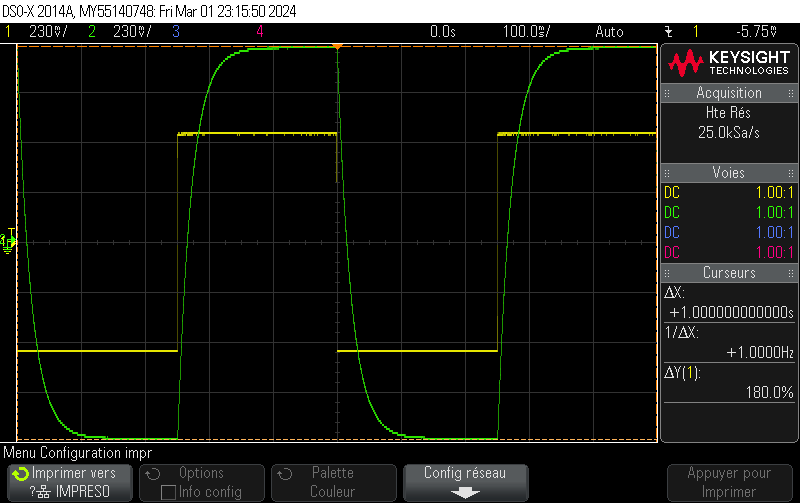
\includegraphics[width=0.75\textwidth]{mesureA1.png}
    \caption{Image de l'oscilloscope lors la mesure de $A$ pour le premiere systeme}
    \label{fig:mesureA1}
\end{figure}

Pour la suite on mesure l'amplification pour les entrées sinusoidales.

Une fois $A$ connue, sachant que la fréquence de 
coupure a $-3 dB$ $f_{-3dB}$ représente
\[
    20 \cdot log(\left | A \right|) - 3dB =  20 \cdot log\left(\left | A \right|\right) + 20 \cdot log \left( \frac{1}{\sqrt{2}} \right)
    = 20 \cdot log \left( \frac{\left| A \right|}{\sqrt{2}} \right)
\]
on sait qu'on cherche une fréquence pour laquelle l'amplitude de la sortie est $S_{-3dB} \simeq  0.7 \cdot A$, autrement dit $70\%$ de l'amplitude 
dans la bande passante. En connaissant $f_{-3dB}$ on peut commencer a mesurer l'amplification (le rapport sortie / entrée) et le 
déphasage de notre systeme, pour des valeur écarté sur l'échelle logarithmique, mais plus sérré
autour la fréquence $f_{-3dB}$. \par

\begin{figure}[h]
    \centering
    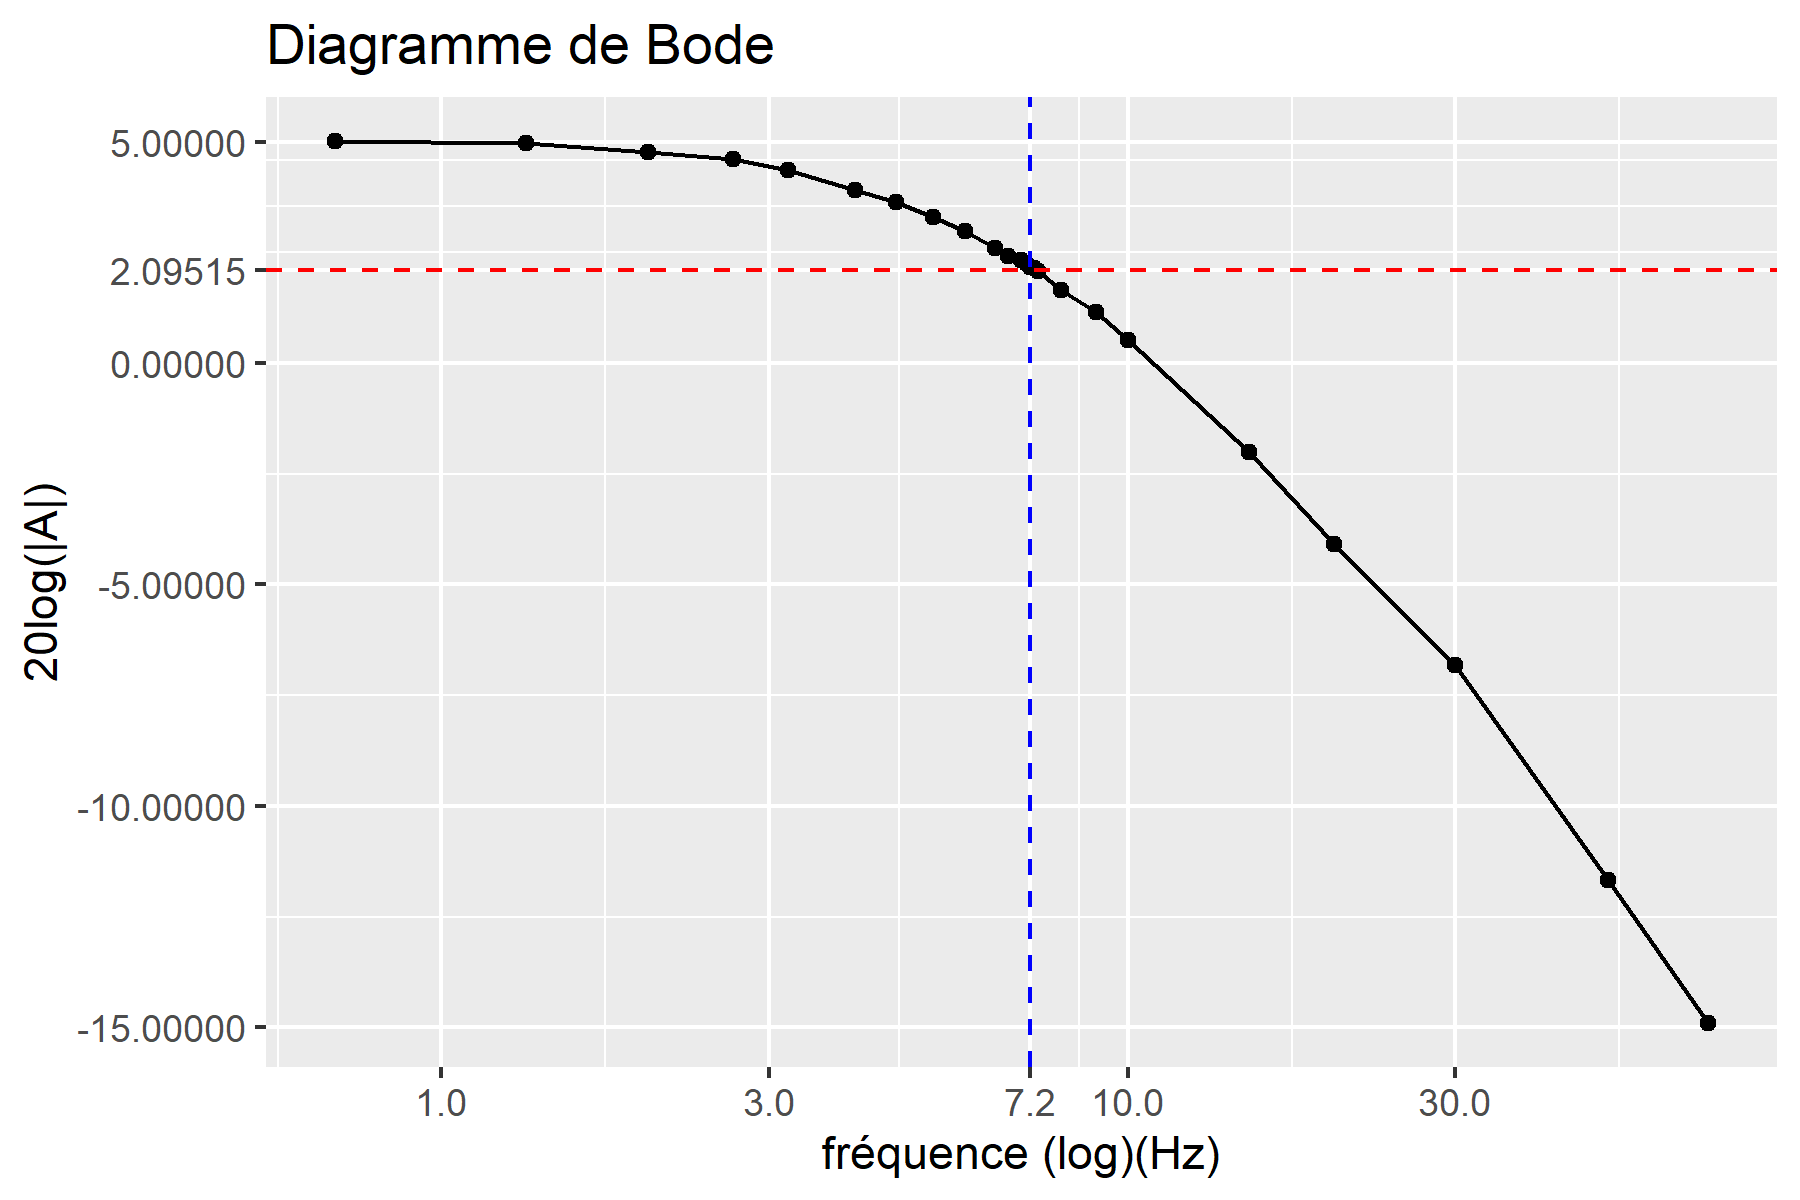
\includegraphics[width=0.75\textwidth]{bode1.png}
    \caption{Diagramme de Bode pour le premiere systeme}
    \label{fig:diagBode1}
\end{figure}

Il est important de noter ici le fait que sur le graphique on a l'impression que
l'intersection des deux droites n'est pas exactement sur la courbe. Il est vrai 
qu'une valeur de $7.4 Hz$ corresponderais mieux sur le graphe pour $f_{-3dB}$ mais 
expérimentalement on a mesuré un déphasage de $-45 \deg$ a une fréquence de $7.2 Hz$, c'est pour 
cela qu'on a décidé de guarder cette valeur.

\begin{figure}[H]
    \centering
    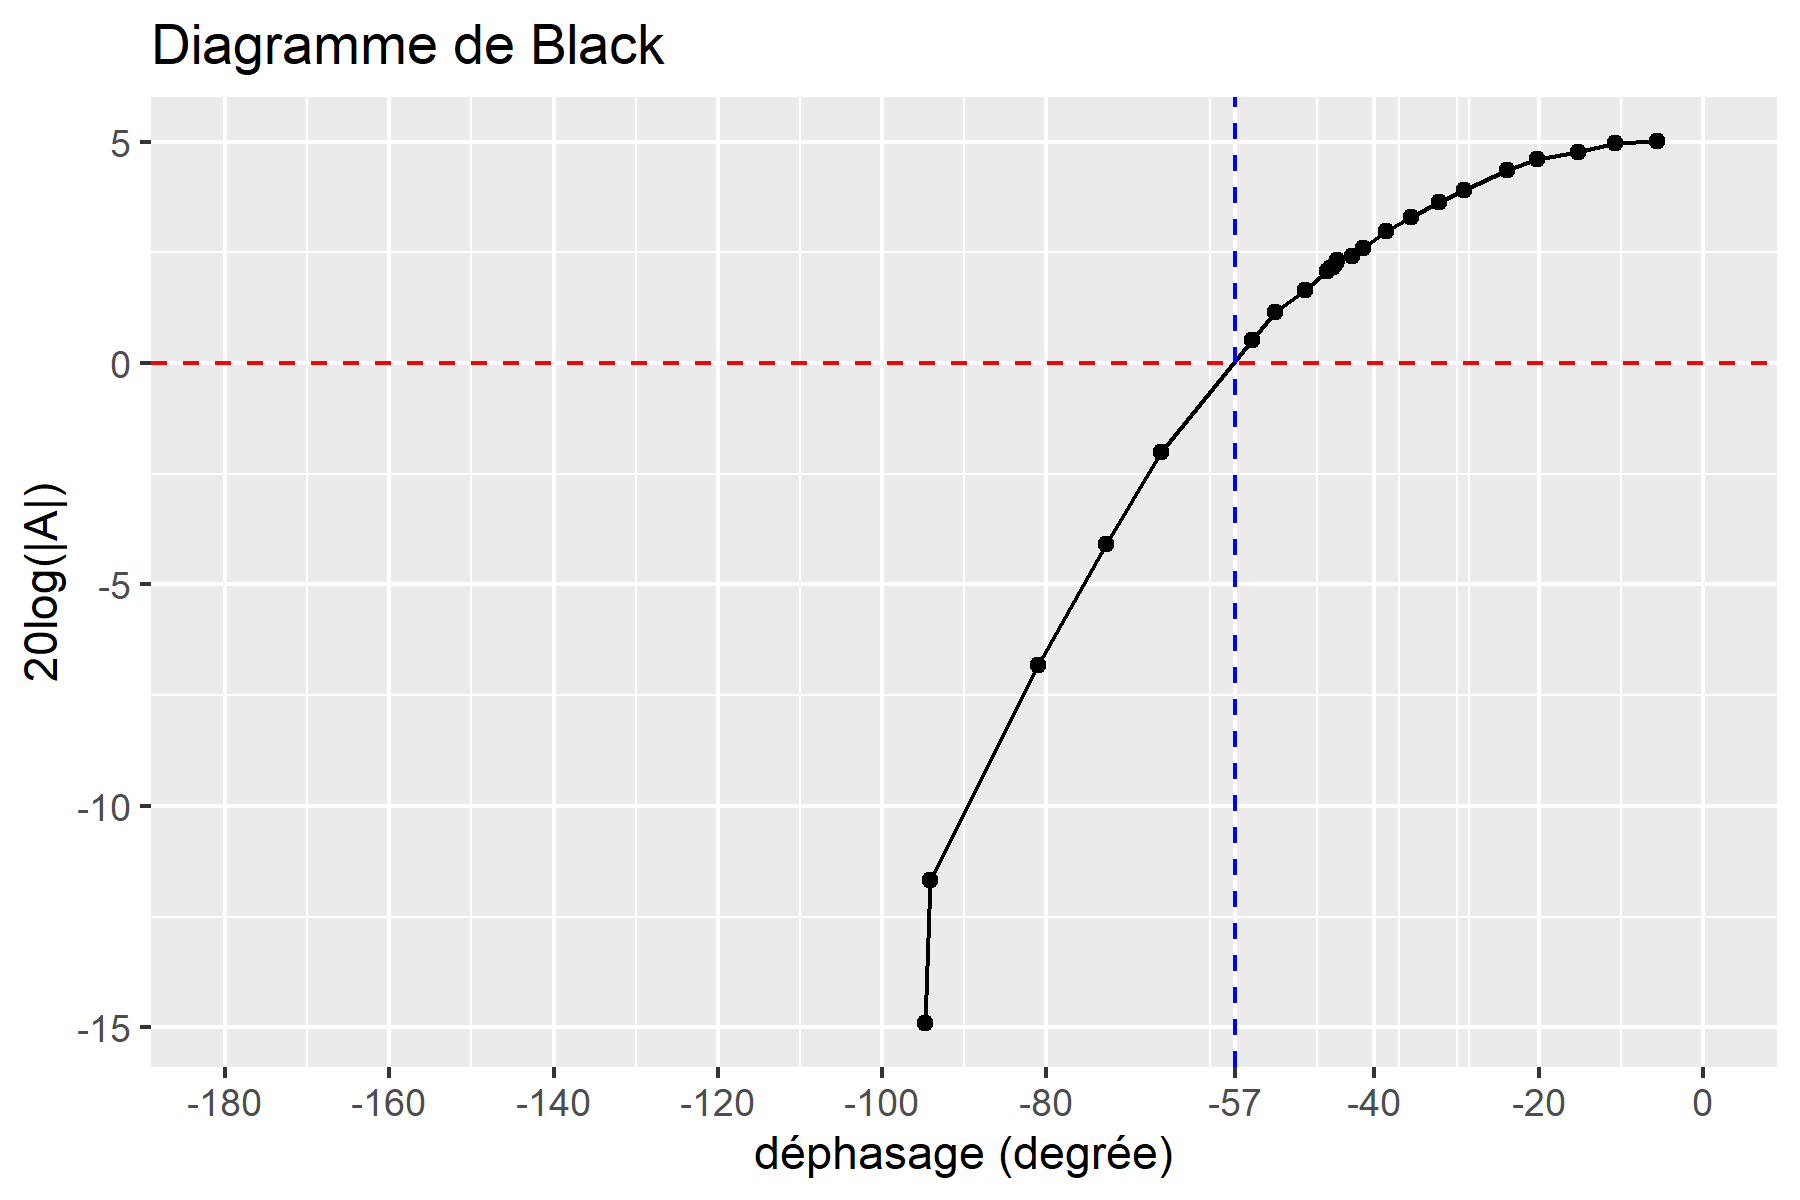
\includegraphics[width=0.75\textwidth]{black1.png}
    \caption{Diagramme de Black pour le premiere systeme}
    \label{fig:diagBlack1}
\end{figure}

Il est possible de déterminer la marge de phase en calculant graphiquement depuis la figure \ref{fig:diagBlack1}
, la difference entre 
$-180$ et le point d'intersection de la courbe avec l'axe des abscisses. Dans notre cas:
\[
    M_{ph} = -57 - (-180) = 123 deg
    \]
La marge de phase est orienté selon les valeurs de l'abscisse croissantes.\par 

En regardant les allures de diagrammes de Black et Bode, on peut remarquer que la modélisatoin du systeme par un systeme d'ordre
1 semble raisonnable.


\subsubsection{Systeme 2}

Pour le systeme 2, on constate qu'en variant la fréquence d'entrée sinusoidale, au début l'amplification augmente, ainsi
nous soupçonnons que le systeme peut pas etre modélisé par un systeme d'ordre 1 puisque ces systemes
ne présentes jamais des résonances. Ainsi on va modéliser le systeme par un systeme d'ordre 2.

Pour une entrée sinusoidale, on mesure la réponse de systeme par rapport a l'entrée ainsi que le déphasage afin d'obtenir 
le diagramme de Bode et de Black:

\begin{figure}[H]
    \centering
    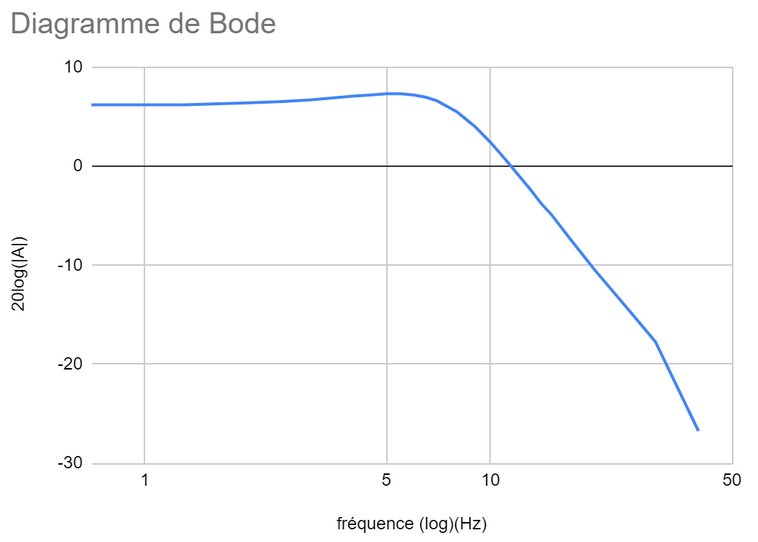
\includegraphics[width=0.75\textwidth]{bode2.png}
    \caption{Diagramme de Bode pour la seconde sortie}
    \label{fig:diagBlack1}
\end{figure}
\begin{figure}[H]
    \centering
    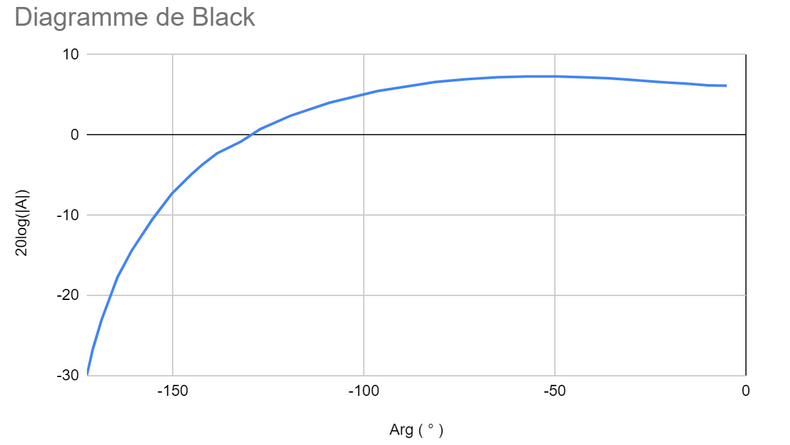
\includegraphics[width=0.75\textwidth]{black2.png}
    \caption{Diagramme de Black pour la seconde sortie}
    \label{fig:diagBlack1}
\end{figure}

Il est possible de déterminer la marge de phase en calculant graphiquement la différence entre -180° et le point d'intersection de la courbe avec l'axe des abscisses. Ici on obtient $M_p = 55deg$
On voit bien sur le diagramme de Bode que la fonction de transfert présente une résonance, ainsi il est plutot réaliste de modéliser
ce systeme par un systeme de seconde ordre.
\section{Réponse indicielle}

\par
Dans cette deuxieme partie on va s'interesser a l'identification des systemes, c'est a dire 
trouver une fonction de transfert, qui décrit au plus proche notre systeme. Il est demandé de tracer
la \textit{caractéristique statique} de notre systeme, qui est la courbe qui représente la sortie
en fonction de l'entrée. Lorsque notre systeme est linéaire, la caractéristique statique est
une droite de pente $A$, l'amplification. En réalité étant donné que le domaine linéaire de la caractéristique statique est
toujours limité (par exemple par la tension de saturation des amplificateurs opérationnelles), c'est a dire 
que la droite n'a pas en tant que limite en $\pm \infty$ l'infini, deux points de cassures, a partir desquelles
la pente devient nulle.

\subsection{Système du première ordre}

Pour les systemes de premiere ordre de type passe-bas, on peut décrire le systeme dans le domaine de Laplace
par la fonction 
\[
    F_{1}(p) = \frac{A}{1 + \tau p}     
\]
ou $A$ représente l'amplification dans la bande passante (pour les passe-bas c'est aussi\\ l'amplification statique, dans ce cas sans unité)
et $\tau$ le constant de temps. Il est ici possible de déterminer l'amplification $A$ en soumettant notre systeme
a une entrée de type échelon de fréquence $f << 10Hz$. Ceci en realité est faite en mettant un signale carré de fréquence faible. Pour mesurer $\tau$ il suffit de mesurer le temps de réponse a 5 pourcent
c'est a dire le temps a partir duquel la réponse est autour de sa valeur en régime permanent en ne plus dépassant $\pm 5\%$ de cette valeur. On peut bien visualiser
le régime permanent et transitoire au meme temps, si on choisit une fréquence telle que le temps de réponse a $5\%$ est égale a la moitié de la demi-période de notre
signale d'entrée:
\[
    \frac{T_{E}}{4} = t_{5\%}
\]
ou $T_{E}$ est la période du signale d'entrée.
\par

\begin{figure}[h]
    \centering
    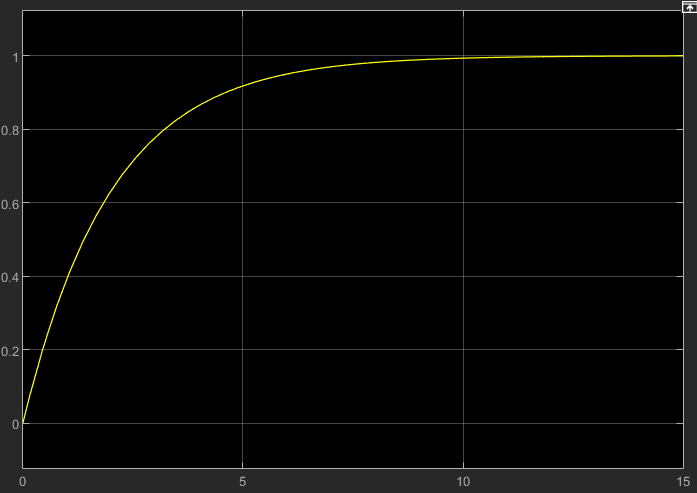
\includegraphics[width=0.75\textwidth]{reponse1erordregenerale.png}
    \caption{Réponse d'un système à première ordre}
    \label{fig:reponse1erordre}
\end{figure}

Lorsqu'on souhaite de mesurer ces caractéristiques avec un entrée harmonique (sinusoidale) on peut soumettre le systeme
a un signale sinusoidale de fréquence basse, et on mesure le rapport des valeurs maximums des allures des sortie par rapport a 
l'entrée. Pour trouver $\tau$ on peut mesurer la fréquence de coupure a $-3dB$ en sachant que 
$f_{-3dB} = 2 \pi \omega_{0}$ donc
\[
    \omega_{0} = \frac{f_{-3dB}}{2 \pi}
\]
Il est maintenant facile a déterminer $\tau$ en connaissant la relation
\[
    \tau = \frac{1}{\omega_{0}}
\]
ou $\omega_{0}$ est la pulsation de cassure a $-3dB$ et aussi la pulsation de coupure vu qu'il s'agit 
d'un systeme du premiere ordre. Voir la figure \ref{fig:reponse1erordre} 
pour voir l'allure de la réponse
d'un tel système.

En appliquant un signale d'entrée constant (en pratique on met un signale carré), on obtient une réponse
comme dans la figure 

\begin{figure}[h]
    \centering
    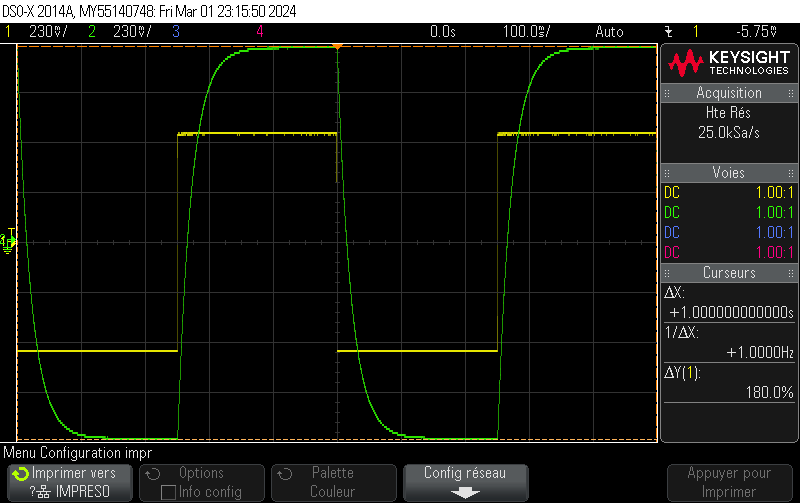
\includegraphics[width=0.75\textwidth]{mesureA1.png}
    \caption{Réponse de systeme 1 de la boite}
    \label{fig:reponse1ersys}
\end{figure}

Le systeme ne présente pas de dépassements et de plus quand le signale d'entrée change de valeur, la pente
en la réponse n'est pas nulle, ainsi il est raisonnable de modéliser ce systeme par un systeme de premiere ordre.
On est alors capable de mesurer l'amplification (déja fait, $A = 1.8$) et le temps de réponse afin d'obtenir le constant de temps $\tau$
sachant que le temps de réponse a $5\%$ est égale a 3 fois $\tau$. On obtient alors $\tau = 0.021667$, d'ou on propose comme modele:
\[
    F_1(p) = \frac{1.8}{1 + 0.021667p}  
\]

On remarque que le systeme est stable, avec une valeur finale de $1.8$ fois l'entrée. En le mesurant pour plusieur valeurs,
on est capable de tracer la caractéristique statique de ce systeme, en représentant la valeur en régime permanent de la sortie par rapport 
a la valeur de l'entrée:

\begin{figure}[H]
    \centering
    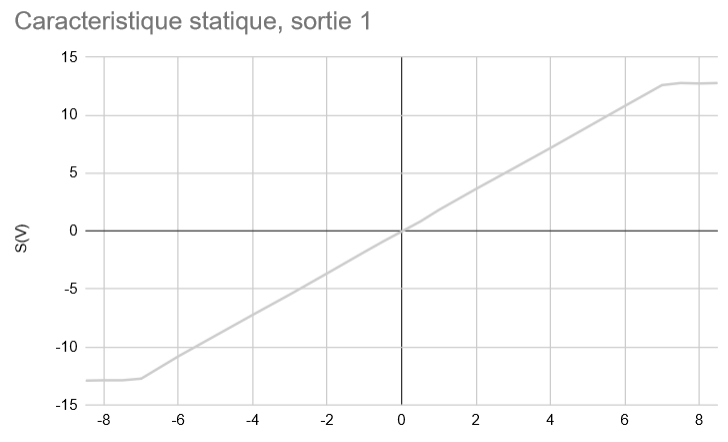
\includegraphics[width=0.75\textwidth]{caracteristiquestatiquesys1.png}
    \caption{Caractéristique statique systeme 1}
    \label{fig:carstattiquesys1}
\end{figure}

On en déduit que la zone de linéarité de ce systeme est entre $\pm 7$. Avec les valeurs spécifiques on est capable de déterminer
la valeur de la pente de la droite dans la zone linéaire, qui est autour de $1.8$ pour ce systeme qui est l'amplification dans la bande passante de notre systeme.

\subsection{Système du second ordre}

Les systèmes du second ordre de type passe-bas peuvent être décrit dans le domaine de Laplace par 
la fonction

\[
  F_{2} (p) =   \frac{A}{1 + 2m \frac{p}{\omega_{0}} + \left( \frac{p}{\omega_{0}} \right)^2}
\]

ou $A$ est l'amplification dans la bande passante (pour les passe bas l'amplification statique aussi), 
$m$ est le \textit{coefficient d'amortissement} et $\omega_{0}$ est la pulsation de cassure de la fonction de 
transfert. Lorsque le coefficient d'amortissement est inférieur à $\frac{1}{\sqrt{2}}$, la réponse du système présente
des \textit{dépassements}, c'est a dire que la réponse prend des valeurs supérieurs à la valeur en régime permanent.


\begin{figure}[h]
    \begin{subfigure}[h!]{0.4\linewidth}
    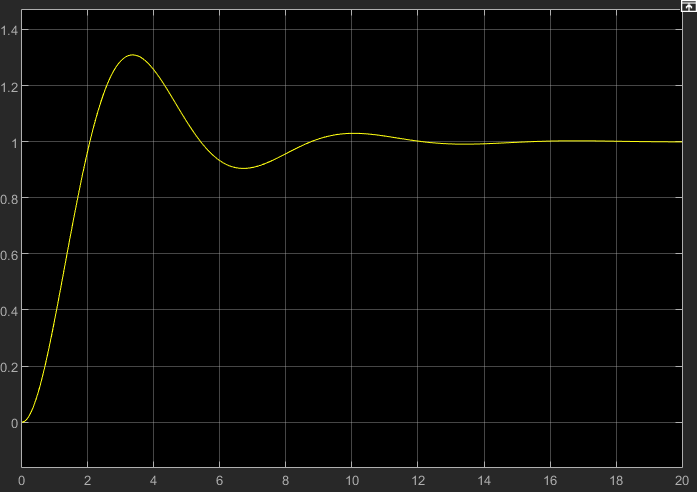
\includegraphics[width=\linewidth]{reponse2ndordresmallz.png}
    \caption{$0 < m < 1$}
    \end{subfigure}
    \hfill
    \begin{subfigure}[h!]{0.4\linewidth}
    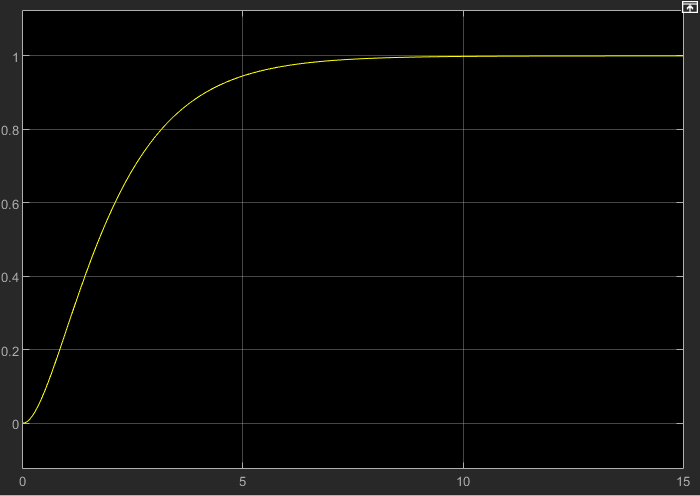
\includegraphics[width=\linewidth]{reponse2ndordrebigz.png}
    \caption{$m > 1$}
    \end{subfigure}
    \caption{Réponse d'un système a 2nd ordre}
\end{figure}

Dans le cas ou $m < 1$, afin de mesurer l'amplification dans la bande passante $A$ on peut mesurer
la réponse a un échelon en boucle ouverte et comparer le résultat obtenu par rapport a l'entrée. Alors $A = \frac{\Delta S}{\Delta E}$ (ainsi sans unité).
Toujours pour une entrée type échelon, on peut mesurer la premiere dépassement, en prenant la valeur en régime permanent en tant que $100\%$ 
et mesurant le pique de la premiere dépassement. En ce connaissant, on peut déterminer le coefficient d'amortissement $m$ en utilisant les abaques.
On peut également mesurer le temps de réponse a $5\%$ qui est le temps ou l'allure de la réponse entre pour la derniere fois dans la bande
de la valeur en régime permanent $\pm 5\%$ et n'en sors plus. En connaissant déja la valeur du coefficient d'amortissement, on peut utiliser les abaques pour 
déterminer $\omega_0$.

Lorsqu'on prends $F_2(j\omega_0)$ on obtient:

\[
    \frac{A}{1 + 2mj - 1} = \frac{A}{2mj}
\]

d'ou

\[
    |F_2(j\omega_0)| = \frac{|A|}{|2mj|} = \frac{A}{2m}, \quad   \quad Arg(F_2(j\omega_0)) = Arg(\frac{A}{2mj}) = Arg(A) - Arg(2mj) = -\frac{\pi}{2}
\]

Ainsi pour un essai harmonique, lorsqu'on retrouve la fréquence $f$ ou le déphasage est $-\frac{\pi}{2}rad$ on retrouve $\omega_0 = \frac{2\pi}{f}$, 
En mesurant la réponse (soit $v_0$ la valeur mesurée) en cette fréquence on peut déduire que $v_0 = \frac{A}{2m} \Rightarrow m = \frac{A}{2v_0}$.

Pour notre systeme on applique un signale type échelon sur l'entrée. On obtient l'allure suivante:

\begin{figure}[H]
    \centering
    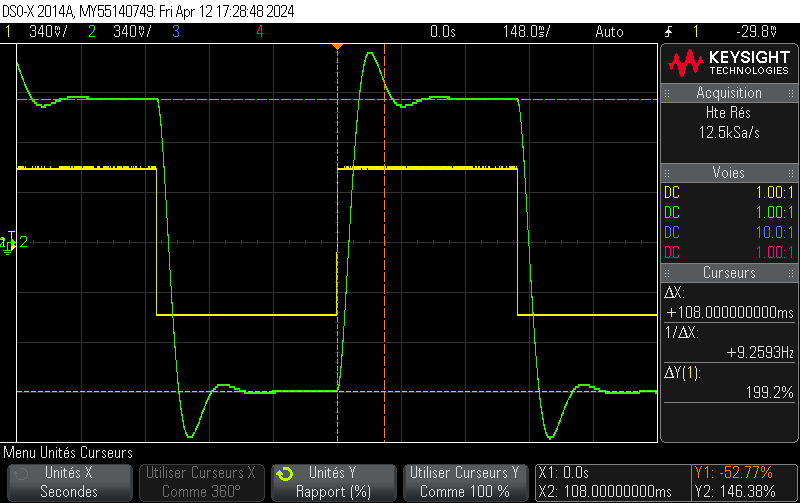
\includegraphics[width=0.75\textwidth]{secondsortiemesureA.png}
    \caption{Mesure de A second sortie}
    \label{fig:mesureA2}
\end{figure}

On peut mesurer la valeur en régime de la réponse par rapport a l'entrée, ici on obtient $A = 2$. En ce faisant pour des
valeurs différentes d'entrée on peut, comme pour le premiere systeme, obtenir la caractéristique statique:

\begin{figure}[H]
    \centering
    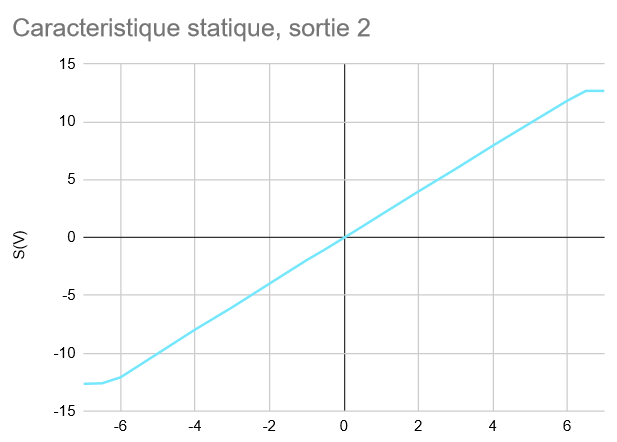
\includegraphics[width=0.75\textwidth]{caracteristiquestatiquesys2.png}
    \caption{Caractéristique statique sortie 2}
    \label{fig:carstattiquesys2}
\end{figure}

Cette caractéristique nous donne une pente proche de $2$ qui est notre amplification dans la bande passante et 
on remarque que la zone de linéarité est entre autour $\pm 6.5 V$.

Depuis le figure \ref{fig:mesureA2} on remarque que le systeme présente des dépassement, ainsi excluant la possibilité
de modéliser le systeme par un systeme de premiere ordre. On remarque également que la pente n'est pas nulle la ou l'entrée bascule.
C'est pour ces raisons la, qu'on propose d'étudier ce systeme comme un systeme de second ordre. On peut alors mesurer ces caractéristiques ($A = 2$ déja fait).
Le systeme soit alors de forme:

\[
    \frac{A}{1 + 2m\frac{p}{\omega_0} + \left( \frac{p}{\omega_0} \right)^2}  
\]

On peut chercher le coefficient d'amortissement $m$, en mesurant la valeur de la premiere dépassement:

\begin{figure}[H]
    \centering
    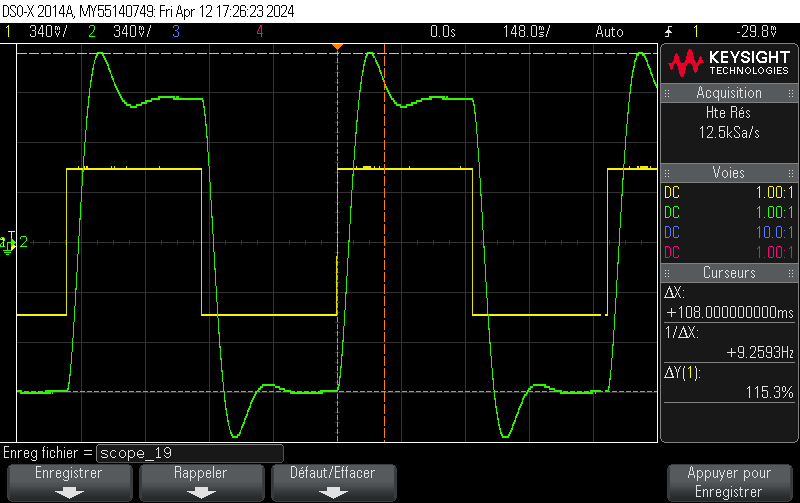
\includegraphics[width=0.75\textwidth]{secondsortie1erdepassementpourcent.png}
    \caption{Mesure de la premiere dépassement}
    \label{fig:1erdepassementsortie2}
\end{figure}

En connaissant ce valeur (dans notre cas $15\%$), on peut utiliser les abaques pour déterminer $m$.
On obtient $m = 0.5$ pour notre systeme. On peut ensuite mesurer le temps de réponse a $5\%$:

\begin{figure}[H]
    \centering
    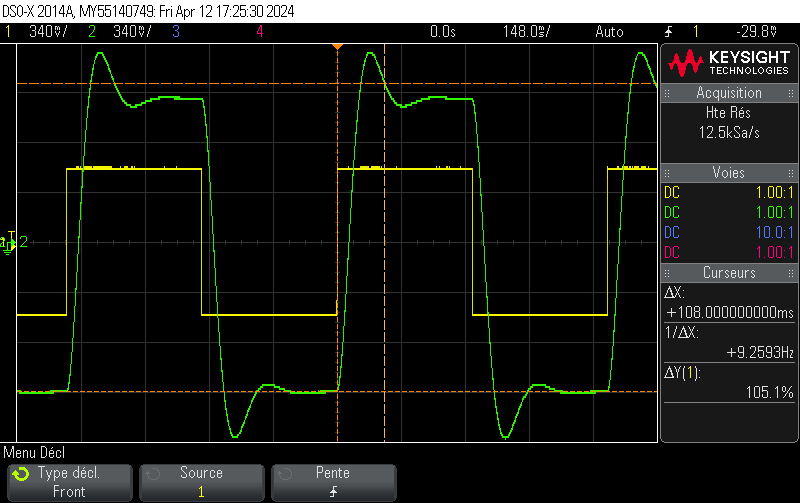
\includegraphics[width=0.75\textwidth]{secondsortietr5pourcent.png}
    \caption{Mesure du temps de réponse}
    \label{fig:tr5prcsortie2}
\end{figure}

En utilisant les abaques, on obtient $t_{r5\%} \cdot \omega_0 = 5$, d'ou 
$\omega_0 = \frac{5}{0.108} = 46.3 rad/s$. Pour la suite, on a pris $\omega_0 = 43.85 rad/s$ puisqu'en refaisant la mesure, on a obtenu une valeur légerement différente pour
le temps de réponse de notre systeme. De ce qui précéde, nous proposons comme modele pour la seconde sortie de la boite:

\[
    F_2(p) = \frac{2}{0.00052p^2 + 0.0228p + 1}
\]

\section{Asservissement des systemes}

\begin{figure}[h]
    \centering
    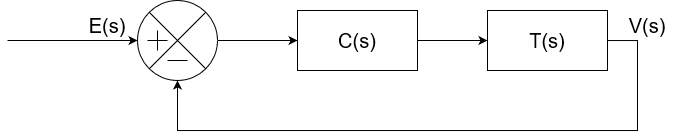
\includegraphics[width=0.75\textwidth]{schemablock2.png}
    \caption{Modélisation par schéma-blocks}
    \label{fig:schemablock}
\end{figure}

Dans cette partie on s'interessera a calculer des correcteurs
pour les systèmes qui permettent de les asservir. On utilisera le logiciel 
MatLab afin de simuler la réponse des systèmes pour pouvoir comparer dans le chapiter 
prochaine aux systèmes réalisés. Les systèmes asservis peuvent etre modélisés
par des schéma-blocks comme représenté sur le figure \ref{fig:schemablock}
, ou $E(s)$ est le signale
d'entrée représenté en domaine de Laplace, $C(s)$ est 
la fonction qui représente le correcteur utilisé et $T(s)$ est la fonction de transfert
de notre système. On peut également représenter sur le schéma, $V(s)$ qui est la sortie
du système en domaine de Laplace.
 



\subsection{Système 1}
Le premiere système peut etre modelisé par un système de premier ordre:
$$
    T(s) = F_1(s) = \frac{A}{1 + \tau s}
$$
ou $A = 1,8$ et $\tau = 21,667$ms d'apres les mesure effectués dans la premiere partie.

\subsubsection{Correction avec correcteur proportionnel}
Pour un correcteur proportionnel on a $C(s) = K, \ K > 0$. Ainsi la fonction de transfert 
en boucle fermée est, d'apres le formule de Black:

\[
    FTBF = \frac{FTBO}{1 + FTBO} = F_{p1}(s)
\]
\[
    F_{p1}(s) = \frac{\frac{KA}{1 + \tau s}}{1 + \frac{KA}{1 + \tau s}} = \frac{KA}{1 + \tau s + KA}    
\]
\[
    F_{p1}(s) = \frac{\frac{KA}{1 + KA}}{1 + \frac{\tau}{1 + KA} s} = \frac{K_{BF}}{1 + \tau_{BF}s}
\]

avec $K_{BF} = \frac{KA}{1 + KA}$ et $\tau_{BF} = \frac{\tau}{1 + KA}$

Il est alors possible de déterminer \textit{l'erreur statique} $\varepsilon_s$ et le 
temps de réponse a $5\%$ $t_{r5\%}$ en fonction de $K$. En effet:

\[
    \varepsilon_s = \lim_{t \rightarrow \infty} \varepsilon(t) = \lim_{s \rightarrow 0} s\cdot \varepsilon(s)
\]
avec $\frac{\varepsilon(s)}{E(s)} = \frac{1}{1 + \frac{KA}{1 + \tau s}}$ d'ou $\varepsilon(s) = \frac{E(s)}{1 + \frac{KA}{1 + \tau s}}$ or ici, $E(s)$ est un échelon donc
\[
    \varepsilon_s = \lim_{s \rightarrow 0} s \cdot \frac{\frac{E_0}{s}}{1 + \frac{KA}{1 + \tau s}} = \frac{E_0}{1 + KA} = \frac{E_0}{1 + K_{BO}}
\]
avec $K_{BO} = KA$. On remarque qu'en augmentant K on arrive a diminuer l'erreur statique, mais 
on n'arrivera jamais a l'annuler.

Vu qu'il s'agit d'un système du premiere ordre, on peut exprimer $t_{r5\%1p}$ (temps de réponse a $5\%$ du premiere systeme en boucle fermée avec 
correcteur proportionnel) avec

\[
    t_{r5\%1p} = 3 \tau_{BF} = 3 \cdot \frac{\tau}{1 + K_{BO}}
\]
ainsi on conclue que le temps de réponse a $5\%$ diminue lorsque $K$ augmente, le systeme devient
plus \textit{rapide} et plus \textit{nerveux}.

En faisant l'application numérique avec $K = 1$ on obtient:
\[
    t_{r5\%1p} = 23,214ms \ \ \ \ \varepsilon_s = 0,357 = 35,7\%
\]

\subsubsection{Chercher le $K$ qui convient}
Dans un premier temps, on va chercher la valeur de $K$ tels que notre système admette une
erreur statique de $10\%$
\[
    \varepsilon_{s10\%} =  \frac{E_0}{1 + KA} \Rightarrow K = \frac{E_0}{A\varepsilon_{s10\%}} - \frac{1}{A} = 5
\]
ensuite, on calcule le temps de réponse a $5\%$ 
\[
    t_{r5\%err10} = \frac{3 \tau}{1 + KA} = 6,5ms.
\]
Pour retrouver le $K$ ou l'erreur statique devient $1\%$ on fait le meme calcul:
\[
    \varepsilon_{s1\%} =  \frac{E_0}{1 + KA} \Rightarrow K = \frac{E_0}{A\varepsilon_{s1\%}} - \frac{1}{A} = 55
\]
ainsi donnant un temps de réponse $t_{r5\%err1}$
\[
    t_{r5\%err1} = 0,65ms
\]

Dans un second temps, on cherche le $K$ tels que le temps de réponse a $5\%$ soit
5 fois plus petit par rapport a en boucle ouverte.

On a donc 
\[
    t_{r5\%5x} = \frac{t_{r5\%}}{5} = \frac{3\tau}{1 + KA} \Rightarrow K = \frac{15 \tau}{t_{r5\%} A} - \frac{1}{A} = 2,22
\]
ou l'erreur statique est:
\[
    \varepsilon_{5x} = \frac{E_0}{1 + KA} =  0,20 = 20\%
\]
Il est possible de faire les memes calcules pour obtenir un temps de réponse 50 fois plus rapide:
\[
    t_{r5\%50x} = \frac{t_{r5\%}}{50} \Rightarrow K = \frac{150 \tau}{t_{r5\%} A} - \frac{1}{A} = 27,22
\]
ou l'erreur statique est:
\[
    \varepsilon_{50x} = \frac{E_0}{1 + KA} =  0,020 = 2\%
\]

\subsubsection{Correction avec un correcteur intégral}

Dans le cas d'un correcteur intégral, on a $C(s) = \frac{1}{T_i s}$ ou $T_i$ représente
le constant de temps de l'intégral.
Comme dans la partie précédente, il est possible d'exprimer la fonction de transfert
en boucle fermée par l'aide du formule de Black:

\[
    FTBF = \frac{FTBO}{1 + FTBO}
\]
\[
    F_{i1}(s) = \frac{\frac{1}{T_i s} \frac{A}{1 + \tau s}}{1 + \frac{1}{T_i s} \frac{A}{1 + \tau s}}
\]
\[
    F_{i1}(s) = \frac{A}{T_i s(1 + \tau s) + A} = \frac{A}{A + T_i s + T_i \tau s^2}
\]
\[
    F_{i1}(s) = \frac{1}{1 + \frac{T_i}{A} s + \frac{T_i \tau}{A} s^2}  
\]
On reconnait la forme d'une fonction de transfert du second ordre.
\[
    F_{i1}(s) = \frac{A}{1 + 2m \frac{s}{\omega_{0}} + \left( \frac{p}{\omega_0} \right)^2} \Rightarrow \omega_0 = \sqrt{\frac{A_1}{T_i \tau}},\ m = \frac{T_i\ \omega_0}{2 A_1} = \sqrt{\frac{T_i}{4 A_1 \tau}}
\]

Il est possible de calculer l'erreur statique en utilisant le meme formule que dans la 
partie correction proportionnel:
\[
    \lim_{s \rightarrow 0} s \cdot  \varepsilon_{s2} (s) 
\]
avec
\[
    \varepsilon_{s2}(s) = \frac{1}{1 + \frac{1}{1 + \frac{T_i}{A_1}s + \frac{T_i \tau}{A_1} s^2}} = \frac{1 + \frac{T_i}{A_1}s + \frac{T_i \tau}{A_1} s^2}{1 + 1 + \frac{T_i}{A_1}s + \frac{T_i \tau}{A_1} s^2}  
\]
donnant
\[
    \lim_{s \rightarrow 0} s \cdot \frac{1}{2} = 0
\]

L'erreur statique est ainsi égale a 0.

Sachant que
\[
    m = \sqrt{\frac{T_i}{4 A_1 \tau}}  
\]
on peut conclure que plus $T_i$ augmente, plus le coefficient d'amortissement $m$ augmente. Ainsi lorsque $T_i$
est assez petit, $m$ dépasse la valeur de $\frac{1}{\sqrt{2}}$ ou le système va commencer a presenter
des dépassements, au meme temps augmentant la rapidité du système. Plus $T_i$ est petit plus le régime transitoire est longue,
ainsi devenant pratiquement instable apres un certain valeur. Le systeme ainsi devient moins nerveux pour les
valeur plus en plus grandes de $T_i$.

En utilisant les abaques on peut chercher $T_i$ pour que la réponse indicielle
présente un dépassement de $5\%$. En effet on cherche $m = 0,7$. Alors

\[
    0,7 = \sqrt{\frac{T_i}{4 A_1 \tau}} \Rightarrow T_i = 0,7^2 \cdot 4 A_1 \tau = 0,0764  
\]

Pour ce $T_i$ le temps de réponse a $5\%$ peut etre retrouvé en utilisant les abaques:

\[
    t_{r5\%dep5\%} \cdot \omega_0 = 3 \Rightarrow t_{r5\%dep5\%} = \frac{3}{\omega_0} = 0,09s = 90ms
\]

\begin{figure}[H]
    \centering
    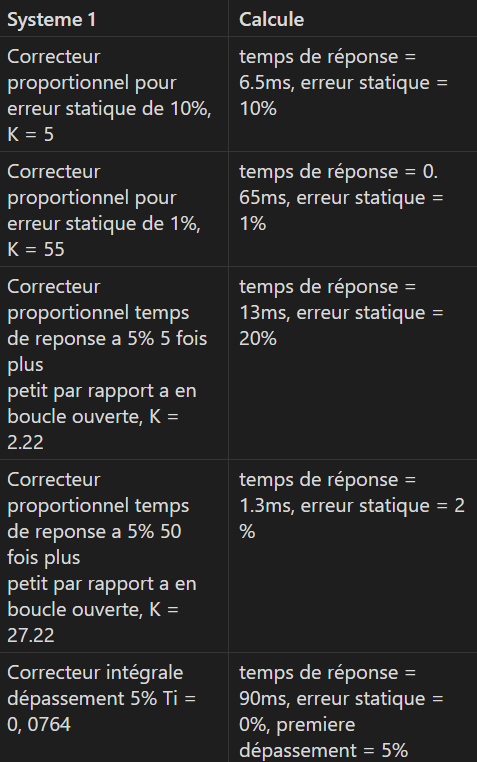
\includegraphics[width=0.75\textwidth]{bilan1.png}
    \caption{Bilan des calcule des correcteurs proportionnels}
\end{figure}

\subsection{Système 2}

Le second système peut etre modelisé par une fonction de transfert du second ordre.

\[
    F_2(s) = \frac{A_2}{1 + 2 m \frac{s}{\omega_0} + \left( \frac{s}{\omega_0}\right)^2}
\]

avec $A_2 = 2$, $m = 0,5$ et $\omega_0 = 43,85$

En utilisant un correcteur proportionnel on obtient:
\[
    F_{p2}(s) = \frac{K_2 \frac{A_2}{1 + 2 m \frac{s}{\omega_0} + \left( \frac{s}{\omega_0}\right)^2}}{1 + K_2 \frac{A_2}{1 + 2 m \frac{s}{\omega_0} + \left( \frac{s}{\omega_0}\right)^2 }} = \frac{K_2 A_2}{1 + K_2A_2 + 2m \frac{s}{\omega_0} + \left( \frac{s}{\omega_0}\right)^2} 
\]

\[
    F_{p2}(s)  = \frac{\frac{K_2A_2}{1 + K_2A_2}}{1 + \frac{2m}{\omega_0(1 + K_2A_2)}s + \frac{1}{1 + K_2A_2} \left( \frac{s}{\omega_0}\right)^2} = \frac{K_{BF2}}{1 + \frac{2m'}{\omega_0'}s + \left( \frac{s}{\omega_0'}\right)^2}
\]
avec $K_{BF2} = \frac{K_2A_2}{1 + K_2A_2}$, $\omega_0' = \omega_0 \sqrt{1 + K_2A_2}$ et $m' = \frac{m}{\sqrt{1 + K_2A_2}}$ on reconnait un système du second ordre. On peut également écrire, vue que $A = 2$,
\[
    K_{BF2} = \frac{2K_2}{1 + 2K_2}, \ \omega_0' = \omega_0 \sqrt{1 + 2K_2},\ m' = \frac{m}{\sqrt{1 + 2K_2}}
\]

On remarque que l'effet d'augmenter $K_2$ est la diminution du coefficient d'amortissement $m'$ qui implique
l'augmentation de la nerveusité du système.

On cherche a calculer $K$ pour obtenir une erreur statique de $10\%$, avec

\[
    \varepsilon_{s2} (s) = \frac{E(s)}{1 + KF_{2}(s)} = \frac{\frac{1}{s}\left(1 + \frac{2m'}{\omega_0'}s + \left( \frac{s}{\omega_0'}\right)^2\right)}{1 + KA_2 + \frac{2m'}{\omega_0'}s + \left( \frac{s}{\omega_0'}\right)^2}
\]
d'ou

$$
    \lim_{s \rightarrow 0} = s \cdot \frac{\frac{1}{s}\left(1 + \frac{2m'}{\omega_0'}s + \left( \frac{s}{\omega_0'}\right)^2\right)}{1 + KA_2 + \frac{2m'}{\omega_0'}s + \left( \frac{s}{\omega_0'}\right)^2} = \frac{1}{1 + KA_2} = 0,1 \Rightarrow K_{10} = 4.5 \\
$$

Il est ainsi possible de déterminer l'amplitude du premiere dépassement, en calculant le coefficient
d'amortissement de la fonction de transfert du systeme en boucle fermée, et regardant les abaques. On retrouve $m'_1 = \frac{m}{\sqrt{1+K_{10}A_2}} = 0.158114$ qui nous laisse montrer depuis les abaques que 
le systeme présente une premiere dépassement de $60\%$. On également calculer le temps de réponse a $5\%$ une fois qu'on calcule $\omega'_{10} = \omega_0 \sqrt{1 + K_{10}A_2} = 138.665$. Depuis les abaques, pour $m = 0.15$, $t_{r5\%}\omega_0 = 20$
, d'ou $t_{r5\%} = 0.144s$


De meme facon on peut retrouver pour une erreur de $2\%$

$$
\frac{1}{K_{2p}A} = 0.02 \Rightarrow K_{2p} = 24.5
$$
pour lequel:
$$
    m'_{2} = 0.0707
$$
a partir duquel on déduit une premiere dépassement de $80\%$. On cherche alors $\omega'_{2} = \omega_0 \sqrt{1 + K_{2p}A_2} = 310.066$, d'ou $t_{r5\%} = \frac{40}{310,0663} = 0.129s$


\section{Simulation des asservissements}

Dans cette partie nous allons simuler la réponse des systemes en utilisant les valeurs
obtenus dans la partie précédente, en utilisant le logiciel l'outil \textit{Simulink} du logiciel \textit{Matlab},
afin de pouvoir les comparer aux résultats de la section précédente.

\subsection{Systeme d'ordre 1}
Dans un premier temps on prends le systeme décrit par la fonction de transfert
$$
    F_{1}(s) = \frac{A}{\tau s + 1}
$$

les valeurs sont $A = 1.8$ et $\tau = 0.021667$.

\subsubsection{Correcteur proportionnel}

Pour les correcteur proportionnel les valeurs obtenus sont 
$$
    K_{sp1.1} = 5 \quad K_{sp1.2} = 55 \quad K_{sp2.1} = 2.22 \quad K_{sp2.2} = 27.22
$$

\begin{figure}[h]
    \centering
    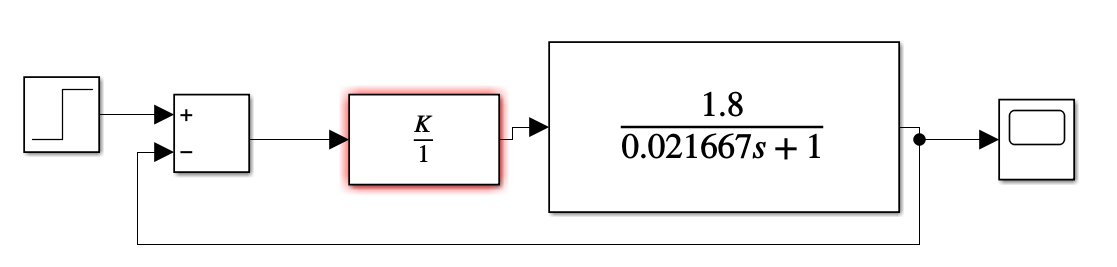
\includegraphics[width=0.75\textwidth]{schemasimulink1.png}
    \caption{Modélisation par schéma-blocks dans Simulink}
    \label{fig:schemablocksim1}
\end{figure}

Dans le logiciel on réalise le schéma de la figure \ref{fig:schemablocksim1} en remplacant K
a chaque fois par les valeurs calculées.


\begin{figure}[h]
    \begin{subfigure}[h!]{0.4\linewidth}
        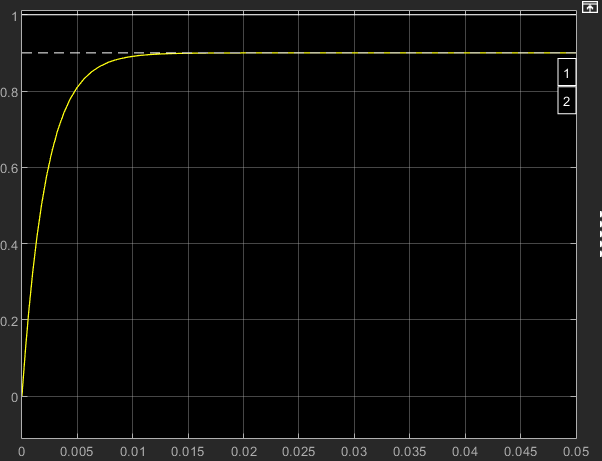
\includegraphics[width=\linewidth]{s1simk5.png}
        \caption{$K_{sp1.1} = 5$}
    \end{subfigure}
    \hfill
    \begin{subfigure}[h!]{0.4\linewidth}
        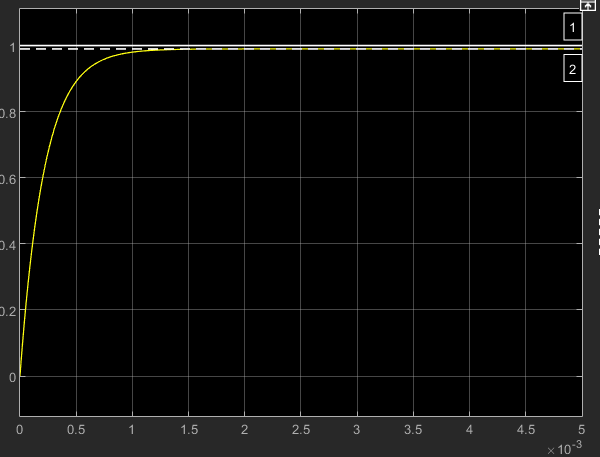
\includegraphics[width=\linewidth]{s1simk55.png}
        \caption{$K_{sp1.2} = 55$}
    \end{subfigure}
    \hfill
    \begin{subfigure}[h!]{0.4\linewidth}
        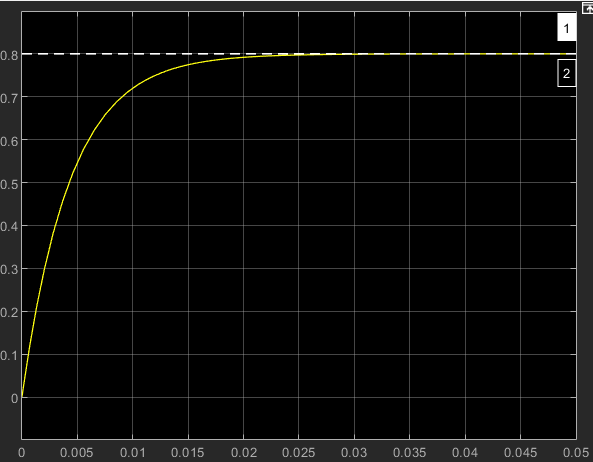
\includegraphics[width=\linewidth]{s1simk2.png}
        \caption{$K_{sp2.1} = 2.22$}
    \end{subfigure}
    \hfill
    \begin{subfigure}[h!]{0.4\linewidth}
        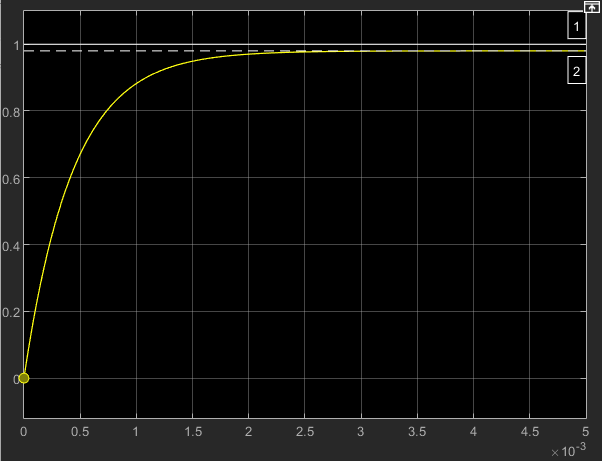
\includegraphics[width=\linewidth]{s1simk27.png}
        \caption{$K_{sp2.2} = 27.22$}
    \end{subfigure}
    \caption{Réponses simulés pour les K différentes, mesure de l'erreur}
\end{figure}

Nos mesures des erreurs statiques sont exactement les que nous avons calculé.

\begin{figure}[H]
    \begin{subfigure}[h!]{0.4\linewidth}
        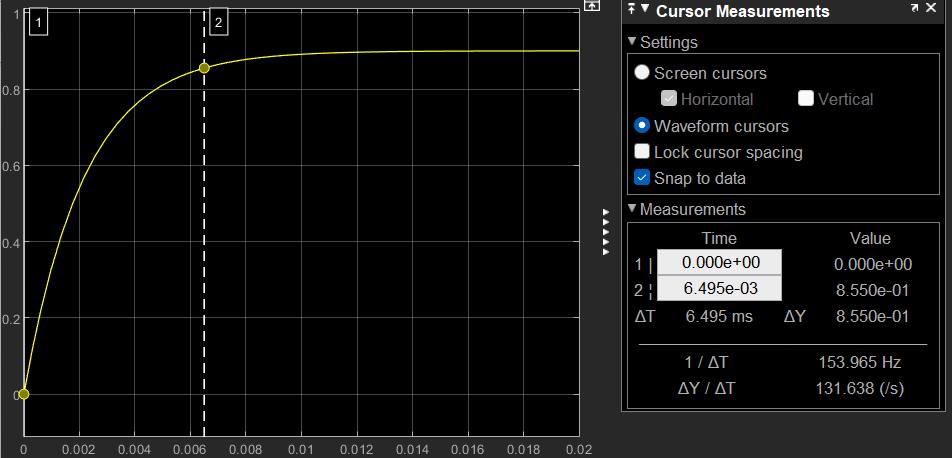
\includegraphics[width=\linewidth]{s1simk5tr.png}
        \caption{$K_{sp1.1} = 5$}
    \end{subfigure}
    \hfill
    \begin{subfigure}[h!]{0.4\linewidth}
        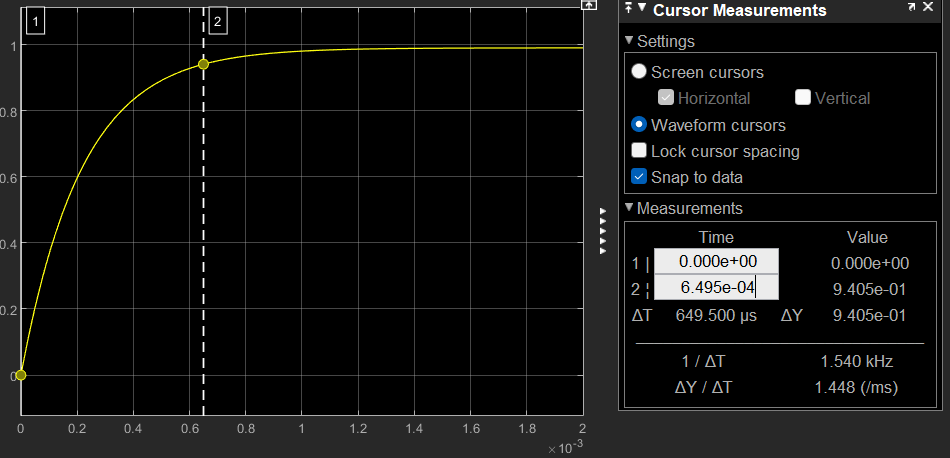
\includegraphics[width=\linewidth]{s1simk55tr.png}
        \caption{$K_{sp1.2} = 55$}
    \end{subfigure}
    \hfill
    \begin{subfigure}[h!]{0.4\linewidth}
        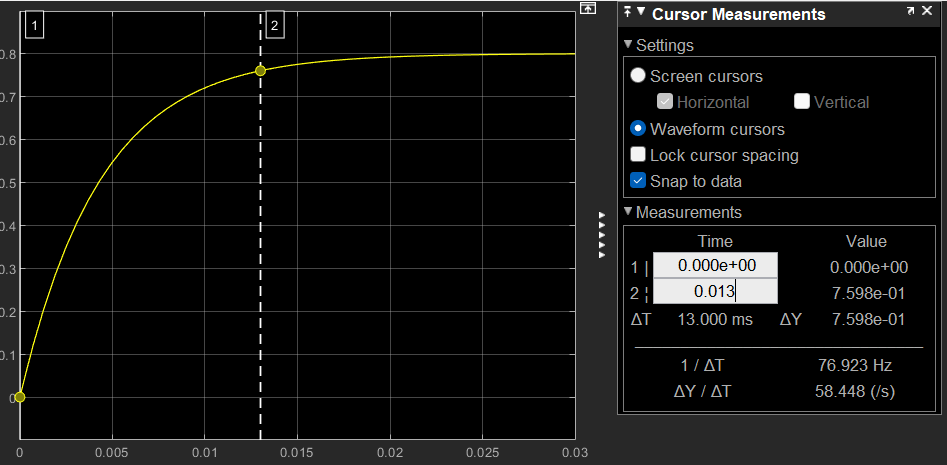
\includegraphics[width=\linewidth]{s1sim2tr.png}
        \caption{$K_{sp2.1} = 2.22$}
    \end{subfigure}
    \hfill
    \begin{subfigure}[h!]{0.4\linewidth}
        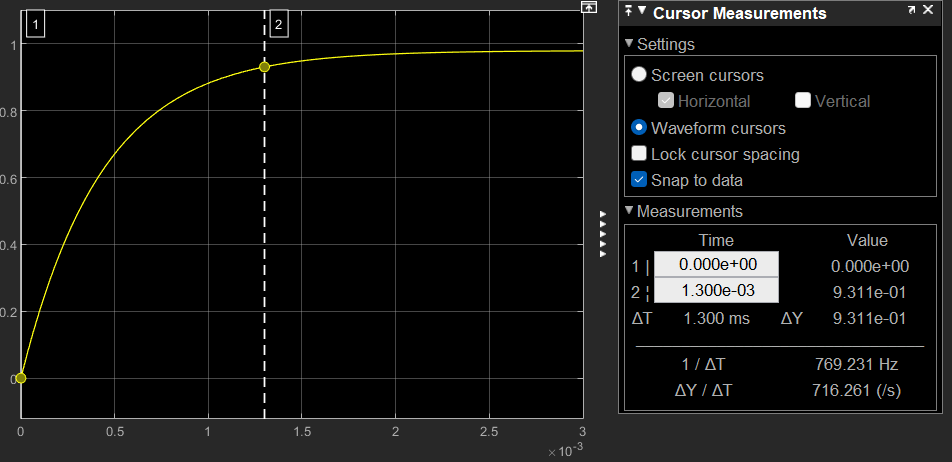
\includegraphics[width=\linewidth]{s1simk27tr.png}
        \caption{$K_{sp2.2} = 27.22$}
    \end{subfigure}
    \caption{Réponses simulés, mesure du temps de réponse}
\end{figure}

Les valeurs sont, si pas exactement les meme, tres proches des valeurs calculés. On peut alors
conclure que les calculs de $K$ sont justes pour vérifier les caractéristiques attendues. On peut également remarquer
le fait que, lorsqu'on augmente $K$, la précision du systeme augmente, c'est a dire que l'erreur statique
diminue, et la rapidité du systeme augmente, c'est a dire que la valeur en régime permanent est atteinte dans moins de temps
que pour les valeurs plus faibles de $K$ (voir les figures).

\subsubsection{Correcteur intégral}

Pour cette section on va simuler le systeme avec un correcteur proportionnel. On modélisera dans Simulink
comme dans la figure \ref{fig:schemablocksim2}.

\begin{figure}[h]
    \centering
    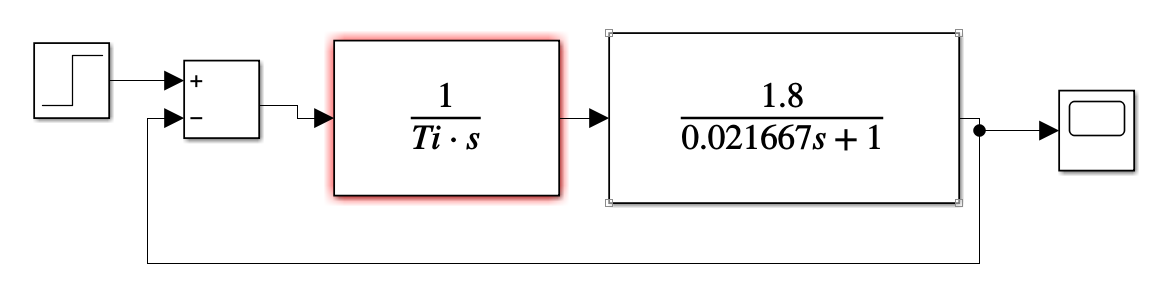
\includegraphics[width=0.75\textwidth]{schemasimulink2.png}
    \caption{Modélisation par schéma-blocks dans Simulink}
    \label{fig:schemablocksim2}
\end{figure}

On prendra les valeurs
$$
    T_{i1} = \tau \quad  T_{i2} = 5\tau \quad  T_{i3} = 10\tau 
$$

\begin{figure}[h]
    \begin{subfigure}[h!]{0.46\linewidth}
        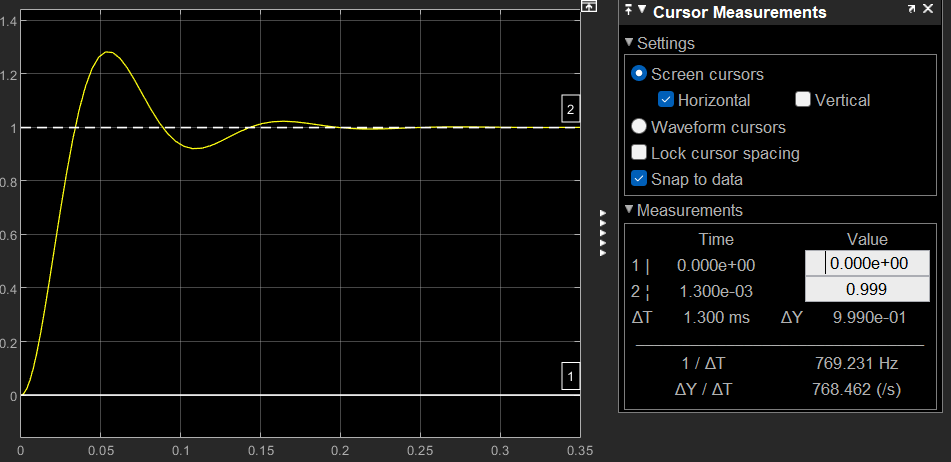
\includegraphics[width=\linewidth]{sim1ti1tauerreur.png}
        \caption{Erreur statique}
    \end{subfigure}
    \hfill
    \begin{subfigure}[h!]{0.46\linewidth}
        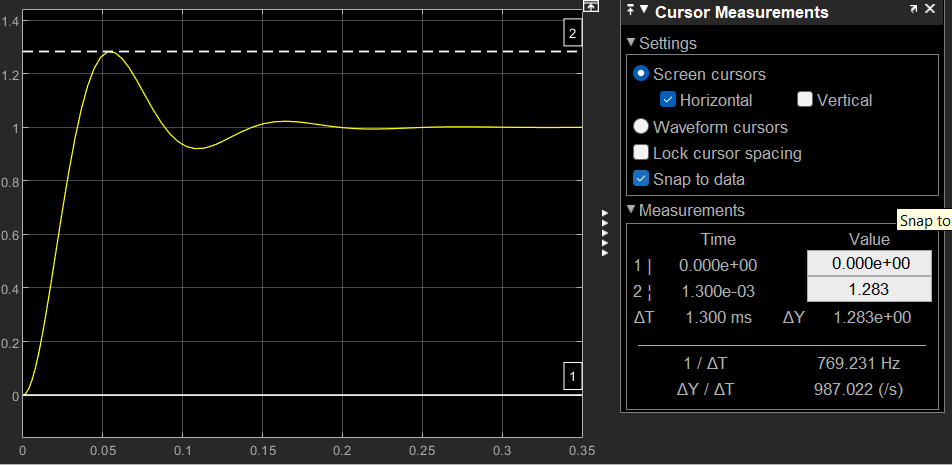
\includegraphics[width=\linewidth]{sim1ti1tau1erdepassement.png}
        \caption{Mesure de premiere dépassement}
    \end{subfigure}
    \hfill
    \begin{subfigure}[h!]{0.46\linewidth}
        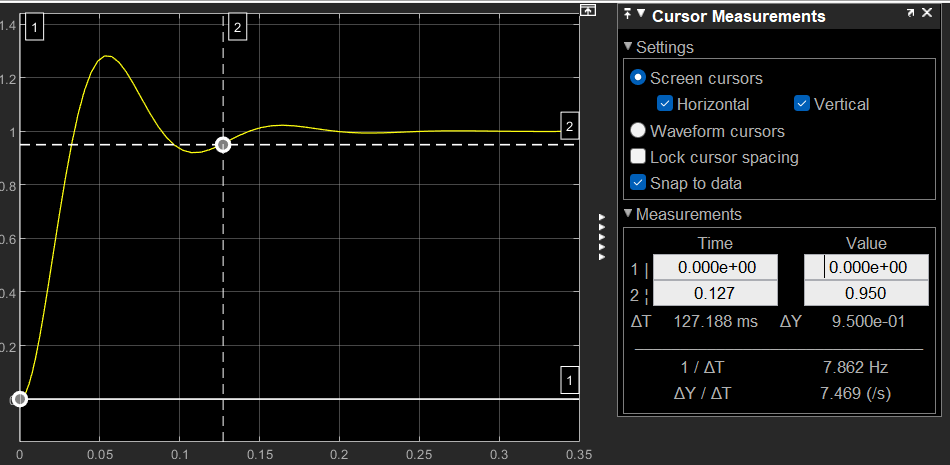
\includegraphics[width=\linewidth]{sim1ti1tautr5prc.png}
        \caption{Mesure du temps de réponse}
    \end{subfigure}
    \caption{Réponses simulés, mesures des caractéristiques pour $T_i = \tau$}
    \label{fig:titau}
\end{figure}

\begin{figure}[H]
    \begin{subfigure}[h!]{0.46\linewidth}
        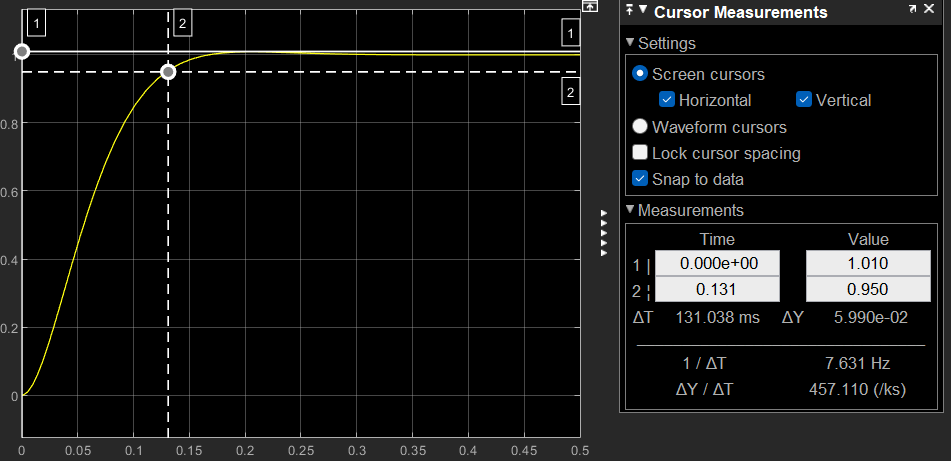
\includegraphics[width=\linewidth]{sim1t5tautr5prc&1erdep.png}
        \caption{Premiere dépassement, temps de réponse}
    \end{subfigure}
    \hfill
    \begin{subfigure}[h!]{0.46\linewidth}
        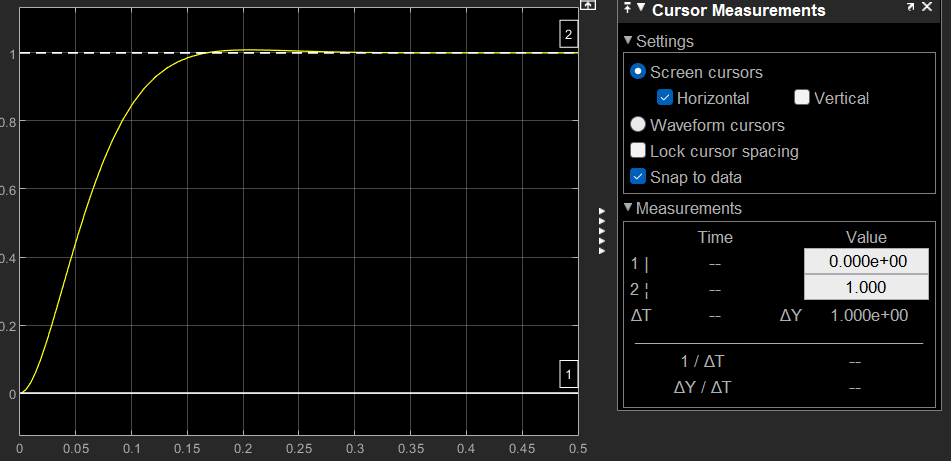
\includegraphics[width=\linewidth]{sim1t5tauerrur.png}
        \caption{Erreur statique}
    \end{subfigure}
    \caption{Réponses simulés, mesures des caractéristiques pour $T_i = 5\tau$}
    \label{fig:ti5tau}
\end{figure}

\begin{figure}[H]
    \begin{subfigure}[h!]{0.46\linewidth}
        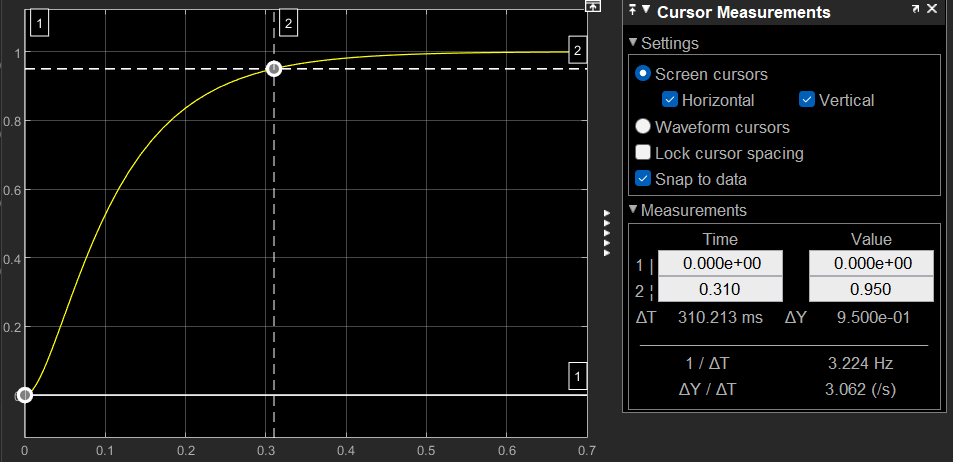
\includegraphics[width=\linewidth]{sim1t10tautr5prc.png}
        \caption{Temps de réponse}
    \end{subfigure}
    \hfill
    \begin{subfigure}[h!]{0.46\linewidth}
        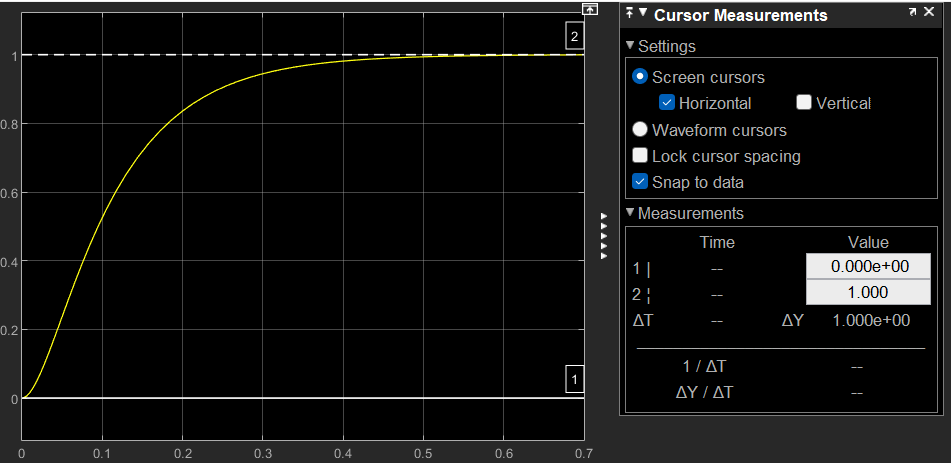
\includegraphics[width=\linewidth]{sim1t10tauerrur.png}
        \caption{Erreur statique}
    \end{subfigure}
    \caption{Réponses simulés, mesures des caractéristiques pour $T_i = 10\tau$}
    \label{fig:ti10tau}
\end{figure}

D'apres les resultats obtenues (figures \ref{fig:titau}, \ref{fig:ti5tau} \ref{fig:ti10tau}), on remarque que 
que nos conclusion de la chapitre précédente sur le changement du dynamique du systeme sont cohérentes: plus la valuer de $T_i$ est grande plus le 
systeme est lant (moins rapide), moins il présente des dépassements. On peut ce conclure grace aux temps de réponses mesurées: pour $T_{i1}$ c'est $127.188 ms$, pour $T_{i2}$ c'est $131.038$ (presque le meme) et pour $T_{i3} $ c'est $310.213 ms$. L'erreur est le meme pour tous les systemes
, c'est 0. Pour ce mesurer, on cherche le nombre

\[
    1 - \frac{\mbox{valeur mesuré en régime permanent}}{\mbox{valeur attendu en régime permanent}} 
\].

La valeur du premier dépassement diminue, ainsi d'apres tout les éléments présentés on peut conclure que le systeme
devient moins nerveux en augmentant $T_i$.

\begin{figure}[H]
    \begin{subfigure}[h!]{0.46\linewidth}
        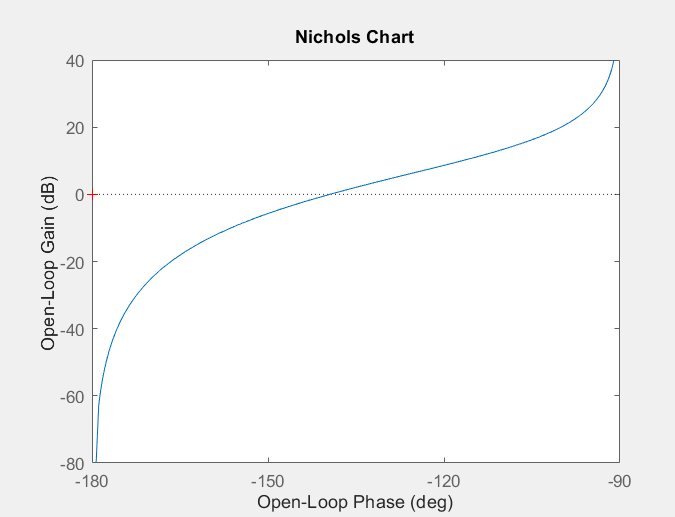
\includegraphics[width=\linewidth]{diagrammblacks1tau1.png}
        \caption{$T_{i1} = \tau$}
    \end{subfigure}
    \hfill
    \begin{subfigure}[h!]{0.46\linewidth}
        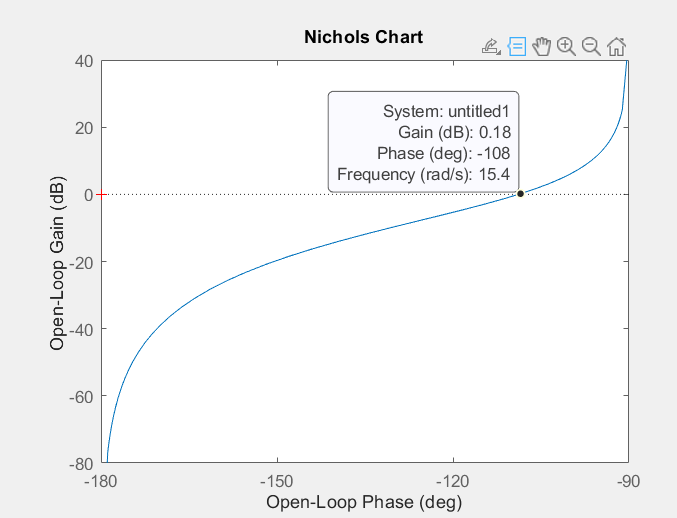
\includegraphics[width=\linewidth]{diagrammblacks1tau5.png}
        \caption{$T_{i2} = 5\tau$}
    \end{subfigure}    
    \hfill
    \begin{subfigure}[h!]{0.46\linewidth}
        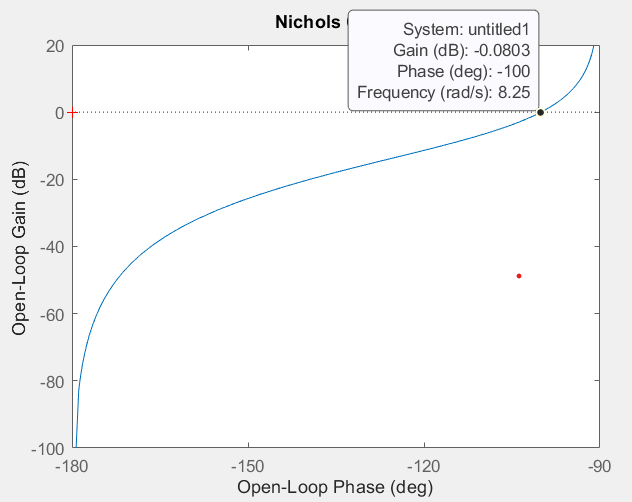
\includegraphics[width=\linewidth]{diagrammblacks1tau10.png}
        \caption{$T_{i3} = 10\tau$}
    \end{subfigure}
    \caption{Diagrammes de black pour les $\tau$ différents}
    \label{fig:diagrammblacks}
\end{figure}

D'après les diagrammes de Black (figures \ref{fig:diagrammblacks}), on peut calculer la \textit{marge de phase}:

\[
    \Delta \Phi_1 = 180 - 139 = 41 deg \quad  \Delta \Phi_2 = 180 - 108 = 72 deg \quad \Delta \Phi_3 = 180 - 100 = 80 deg 
\]

On peut en conclure que plus $\tau$ augmente, plus $T_i$ augmente, plus la marge de phase est grande,
qui implique que la stabilité du systeme augmente si $T_i$ augmente.

\begin{figure}[H]
    \begin{subfigure}[h!]{0.4\linewidth}
        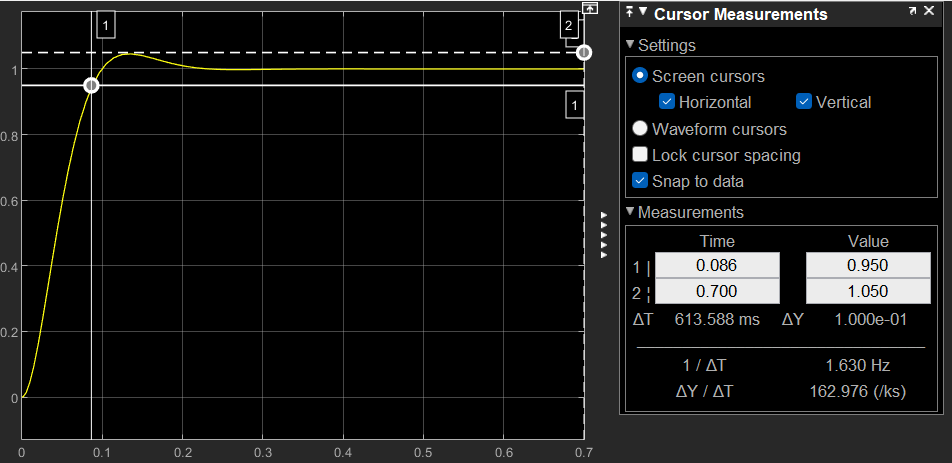
\includegraphics[width=\linewidth]{sim1123tr5prc1erdep.png}
        \caption{Mesure premiere dépassement, temps de réponse}
    \end{subfigure}
    \hfill
    \begin{subfigure}[h!]{0.4\linewidth}
        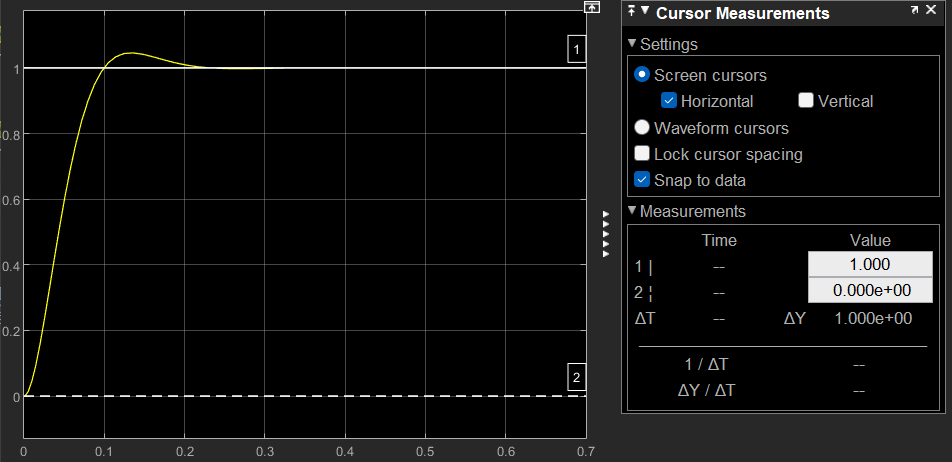
\includegraphics[width=\linewidth]{sim1123erreur.png}
        \caption{Mesure erreur statique}
    \end{subfigure}
    \caption{Simulation avec $T_i = 0.0764$}
    \label{fig:tipour5prc}
\end{figure}

Lorsqu'on applique le $T_i$ trouvé dans la partie précédente pour avoir un premiere dépassement de $5\%$
($T_i = 0.0764$) on mesure un premiere dépassement de $5\%$, un temps de réponse de $86ms$ et une erreur statique nulle (figure \ref{fig:tipour5prc}).
Dans nos calculs de la section précédente, on a trouvé un temps de réponse de $90ms$ donc nos résultats sont cohérentes.

On peut ainsi comparer les résultats des correcteurs proportionnels et intégraux. D'une part, le correcteur
proportionnel ne présente jamais des dépassementes en corrige un système de premier ordre, qui garantit 
que nos composants ne seront pas surchargés. Lorsqu'on augmente la valeur de $K$ pour le correcteur proportionnel 
on augmente, et lorsqu'on augmente $T_i$ du correcteur intégral, on diminue la nerveusité du systeme. Le correcteur proportionnel présente
une erreur statique tendis que l'integral n'en a pas (pour les entrée type échelon).

\begin{figure}[H]
    \centering
    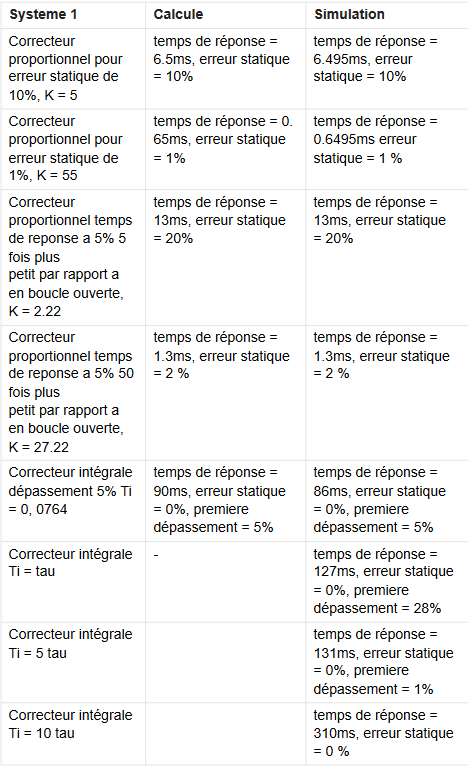
\includegraphics[width=0.75\textwidth]{bilan2.png}
    \caption{Bilan apres simulation}
\end{figure}

\subsection{Systeme d'ordre 2}

\subsubsection{Correcteur proportionnel}

Dans un premier temps, on va simuler le système 2, modélisé par une fonction de transfert d'ordre 2, avec un correcteur proportionnel. On prendra les valeurs de $K$ trouvés précédamment: $K_{2.1} = 4.5$, $K_{2.2} = 24.5$.

\begin{figure}[H]
    \begin{subfigure}[h!]{0.4\linewidth}
        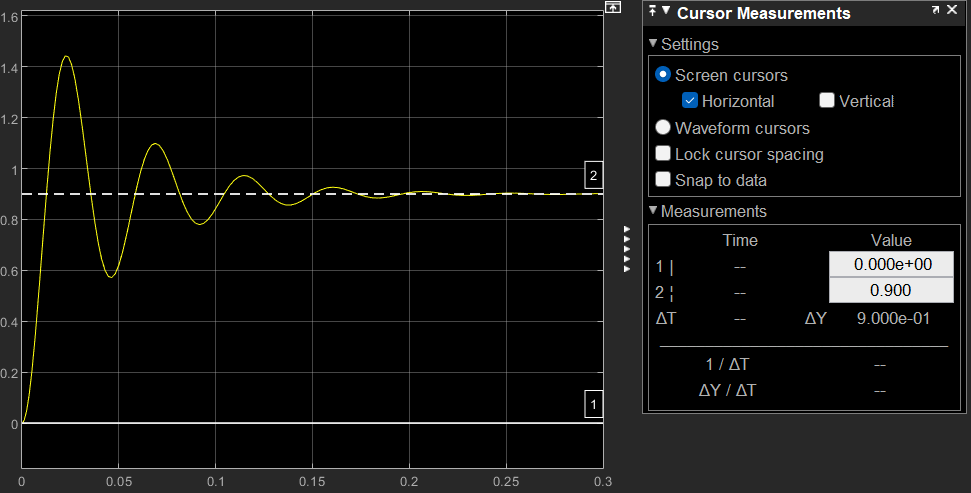
\includegraphics[width=\linewidth]{sim2kpourerreur10prc.png}
        \caption{Erreur statique}
    \end{subfigure}
    \hfill    
    \begin{subfigure}[h!]{0.4\linewidth}
        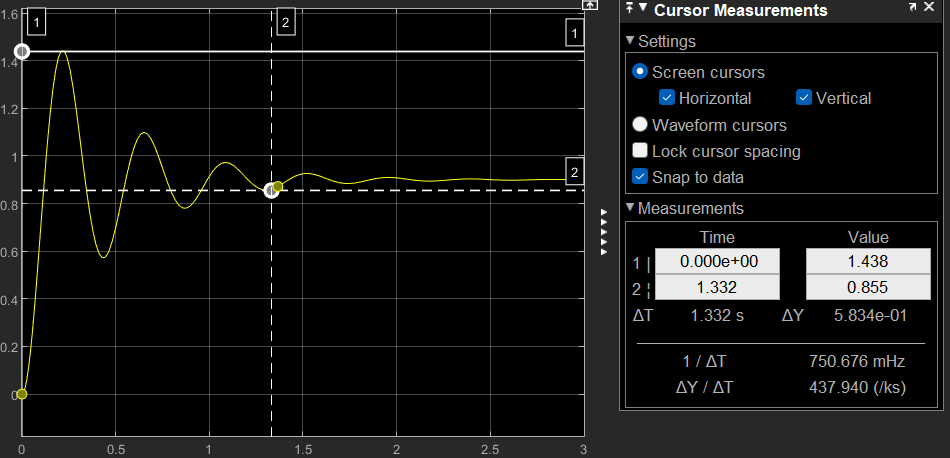
\includegraphics[width=\linewidth]{sim2kpourerreur10prcdeptr.png}
        \caption{Mesure premiere dépassement, temps de réponse}
    \end{subfigure}
    \caption{Simulation avec $K = 4.5$}
    \label{fig:sim2Kpour10prc}
\end{figure}

Pour $K_{2.1} = 4.5$ on trouve une erreur statique de $10\%$, une premiere dépassement de $44.1\%$ et un temps de
réponse a $5\%$ de $0.139s$ ce qui sont cohérentes avec les résultats précédentes (sauf le dépassement [on a trouvé $60\%$ mais mesuré $44.1\%$], la lecture des abaques peut entrainer des erreurs).

\begin{figure}[H]
    \begin{subfigure}[h!]{0.4\linewidth}
        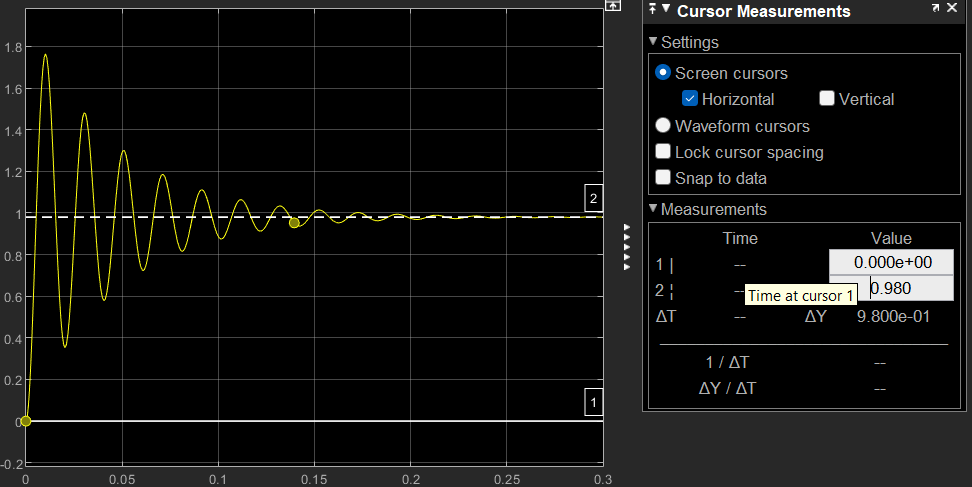
\includegraphics[width=\linewidth]{sim2kpourerreur2prcerreur.png}
        \caption{Erreur statique}
    \end{subfigure}
    \hfill    
    \begin{subfigure}[h!]{0.4\linewidth}
        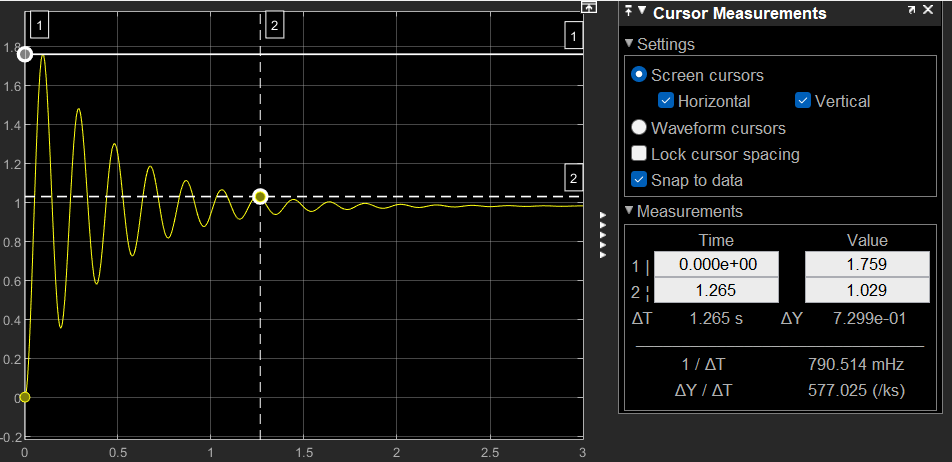
\includegraphics[width=\linewidth]{sim2kpourerreur2prcdeptr.png}
        \caption{Mesure premiere dépassement, temps de réponse}
    \end{subfigure}
    \caption{Simulation avec $K = 24.5$}
    \label{fig:sim2Kpour10prc}
\end{figure}

Pour $K_{2.2} = 24.5$ on retrouve une erreur statique de $2\%$, et on mesure une premiere dépassement de $77.1\%$ et un temps de réponse de 
$0.134s$. Ici les resulats sont plus cohérentes avec celles calculées.

On peut conclure que plus $K$ augmente, plus le système devient nerveux: les premières dépassements sont de plus en plus importants, mais l'erreur statique diminue.
Un premier dépassement de $80 \%\%$ dans le cas de $K_{2.2}$ Peut-être considéré comme trop grand dans certaines applications, ainsi, augmenter la valeur de $K$ afin de 
diminuer l'erreur statique n'est peut etre pas la meilleur solution.

\subsubsection{Correcteur intégral}
On peut dans un second temps regarder l'influence d'un correcteur intégral sur la correction du système. On prendra les valeurs définies dans le TP:

\[
    T_{i1} = 0.456 \quad T_{i2} = 0.22805 \quad T_{i3} = 0.114025 \quad T_{i4} = 0.022805
\]

\begin{figure}[H]
    \begin{subfigure}[h!]{0.4\linewidth}
        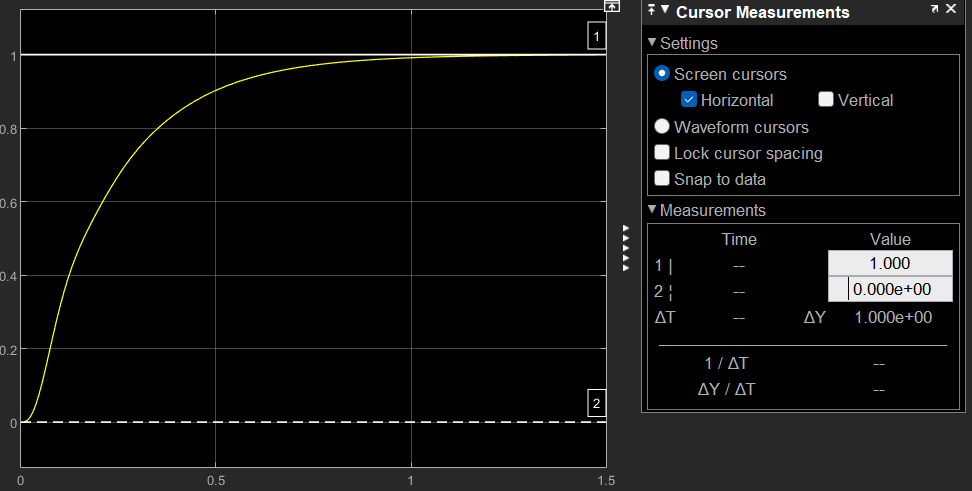
\includegraphics[width=\linewidth]{sim2ti1erreur.png}
        \caption{Erreur statique}
    \end{subfigure}
    \hfill    
    \begin{subfigure}[h!]{0.4\linewidth}
        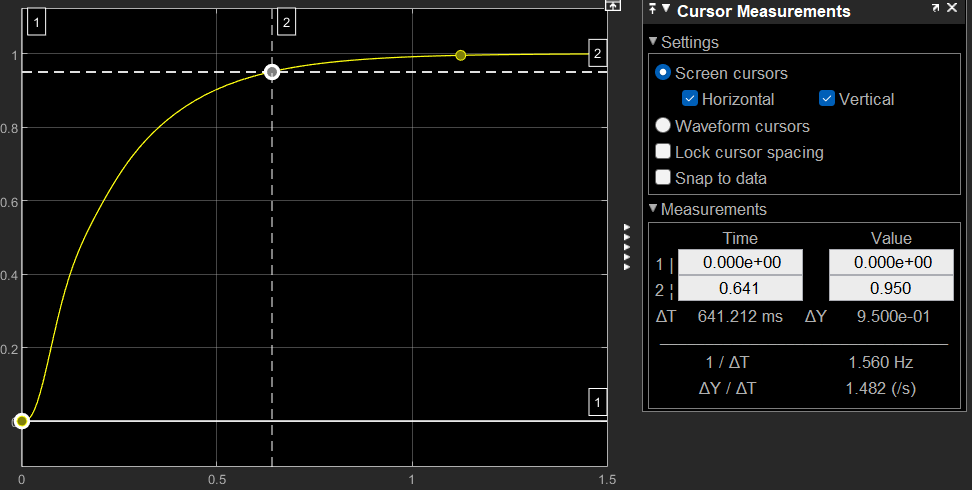
\includegraphics[width=\linewidth]{sim2ti1tr.png}
        \caption{Temps de réponse}
    \end{subfigure}
    \caption{Simulation avec $T_i = 0.456$}
    \label{fig:sim2KTi1}
\end{figure}

\[
    t_{r5\%Ti1} = 0.641s \quad
\]

Pour le premiere $T_i = 0.456$ on retrouve une erreur statique nulle, un temps de réponse de $0.641s$ et il n'y a pas de dépassement.

\begin{figure}[H]
    \begin{subfigure}[h!]{0.4\linewidth}
        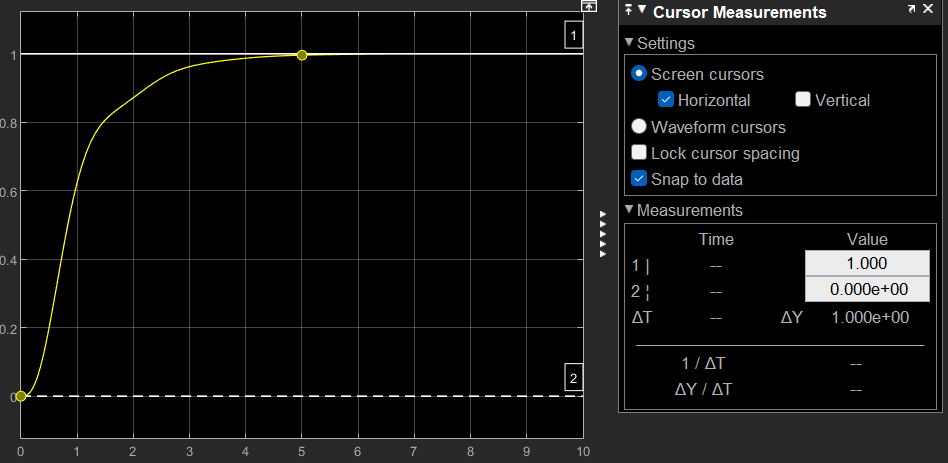
\includegraphics[width=\linewidth]{sim2ti2erreur.png}
        \caption{Erreur statique}
    \end{subfigure}
    \hfill    
    \begin{subfigure}[h!]{0.4\linewidth}
        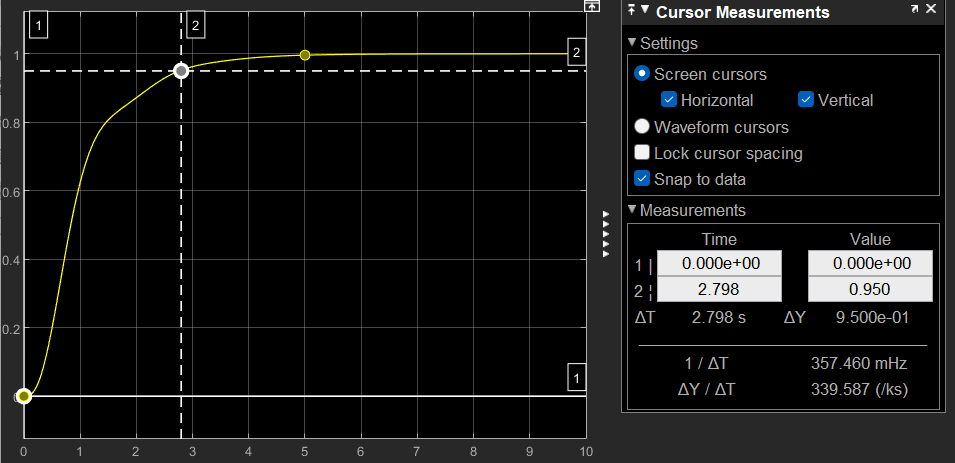
\includegraphics[width=\linewidth]{sim2ti2tr.png}
        \caption{Temps de réponse}
    \end{subfigure}
    \caption{Simulation avec $T_i = 0.22805$}
    \label{fig:sim2KTi2}
\end{figure}

\[
    t_{r5\%Ti2} = 0.298s \quad
\]

Pour $T_i = 0.22805$ on retrouve une erreur statique nulle, un temps de réponse de $ 0.298s$ et il n'y a pas de dépassement.
La rapidité du systeme a augmenté en diminuant la valeur de $T_i$

\begin{figure}[H]
    \begin{subfigure}[h!]{0.4\linewidth}
        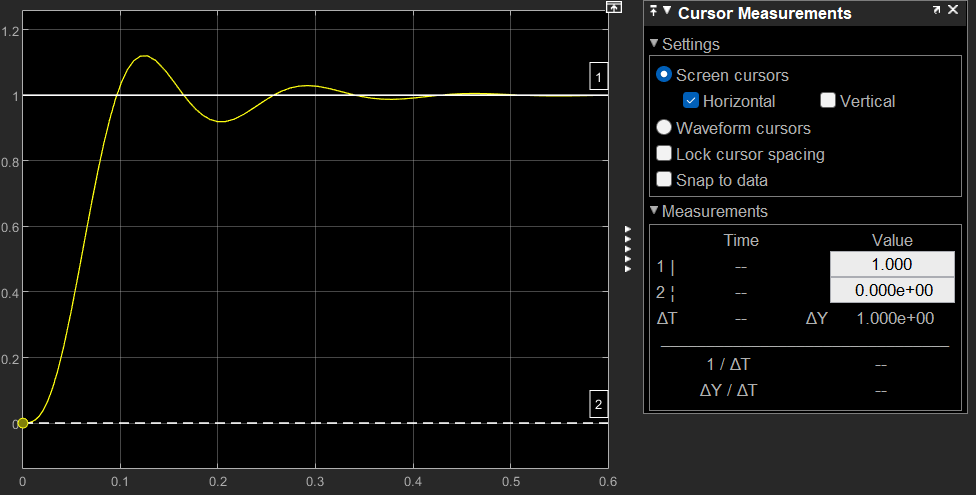
\includegraphics[width=\linewidth]{sim2ti3errur.png}
        \caption{Erreur statique}
    \end{subfigure}
    \hfill    
    \begin{subfigure}[h!]{0.4\linewidth}
        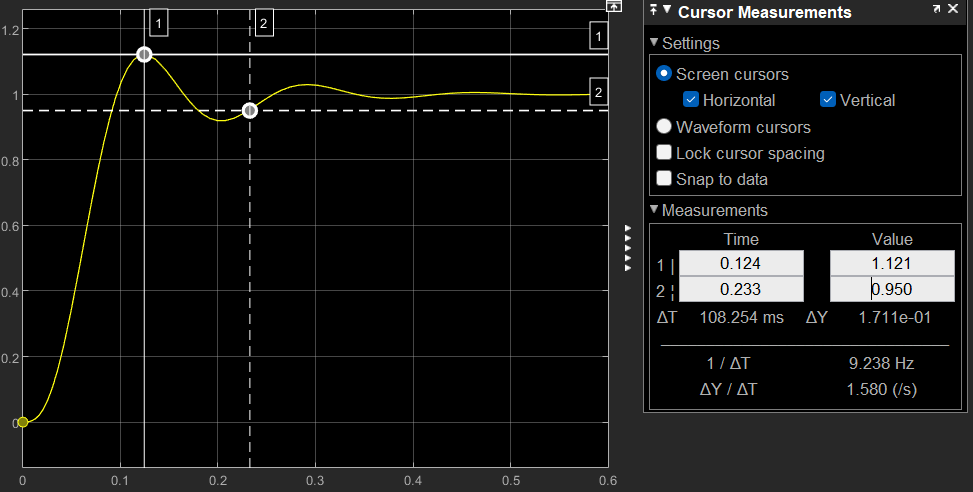
\includegraphics[width=\linewidth]{sim2ti3deptr.png}
        \caption{Temps de réponse, premiere dépassement}
    \end{subfigure}
    \caption{Simulation avec $T_i = 0.114025$}
    \label{fig:sim2KTi3}
\end{figure}

\[
    t_{r5\%Ti3} = 0.233s \quad
\]

Pour $T_i = 0.114025$ on retrouve une erreur statique nulle, un temps de réponse de $0.233s$ et un premier dépassement de
$12.1\%$. On remarque que c'est la nervosité du système qui augmente en diminuant $T_i$, puisque vant il n'y avait pas de dépassement.


\begin{figure}[H]
    \centering
    \begin{subfigure}[h]{0.6\linewidth}
        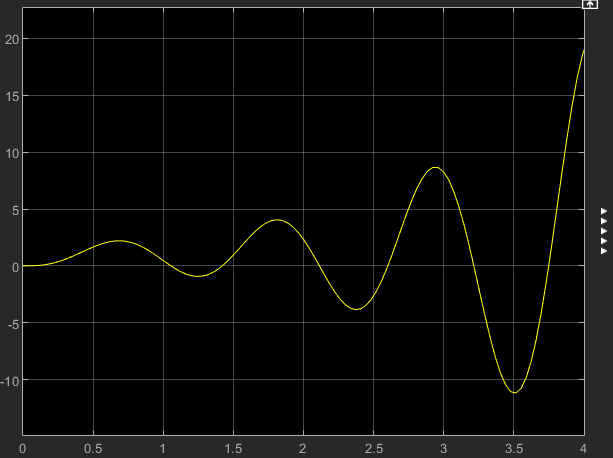
\includegraphics[width=\linewidth]{sim2ti4.png}
        \caption{Systeme instable}
    \end{subfigure}
    \caption{Simulation avec $T_i = 0.215982$}
    \label{fig:sim2KTi4}
\end{figure}

Pour $T_i = 0.022805$ on trouve que le système devient instable. En effet le système n'a pas l'aire de converger vers une valeur 
spécifique, le régime transitoire n'a pas l'aire de se finir.

\begin{figure}[H]
    \begin{subfigure}[h!]{0.4\linewidth}
        \includegraphics[width=\linewidth]{sim2ti1diag.png}
        \caption{$T_i = 0.456$}
    \end{subfigure}
    \hfill    
    \begin{subfigure}[h!]{0.4\linewidth}
        \includegraphics[width=\linewidth]{sim2ti2diag.png}
        \caption{$T_i = 0.22805$}
    \end{subfigure}    
    \hfill    
    \begin{subfigure}[h!]{0.4\linewidth}
        \includegraphics[width=\linewidth]{sim2ti3diag.png}
        \caption{$T_i = 0.114025$}
    \end{subfigure}
    \hfill    
    \begin{subfigure}[h!]{0.4\linewidth}
        \includegraphics[width=\linewidth]{sim2ti4diag.png}
        \caption{$T_i = 0.022805$}
    \end{subfigure}
    \caption{Diagrammes de Black}
    \label{fig:sim2Tiblacks}
\end{figure}

On remarque sur les diagrammes de Black, que plus $T_i$ est grand, plus le système est stable puisque la marge de phase augmente;
mais pour $T_i = 0.022805$ la marge de phase devient négative, ainsi le système n'est pas stable.

\begin{figure}[H]
    \centering
    \includegraphics[width=0.75\textwidth]{bilan3.png}
    \caption{Bilan apres simulation}
\end{figure}

\end{document}
